\section{DFPT - density functional perturbation theory for lattice dynamics and homogeneous electric fields}
\label{Sec:DFPT}

All these DFPT features are written by Honghui Shang and coworkers at FHI, when using routines
related to DFPT, please contact shang@fhi-berlin.mpg.de.

The density functional perturbation theory (DFPT) is in principle the perturbation form of DFT, which is only needed for the second and higher order derivatives ~($2n+1$~theorem). For example, for the calculation of vibrational frequencies and phonon band-structures~(second order derivative) the response of the electronic structure to a nuclear displacement~(first order derivative) is needed. These derivatives can be calculated in the framework of density-functional perturbation theory~(DFPT). DFPT provide access to many fundamental physical phenomena, such as superconductivity, phonon-limited carrier lifetimes in electron transport and hot electron relaxation,  Peierls instabilities, the renormalization of the electronic structure due to nuclear motion,  Born effective charges, phonon-assisted transitions in spectroscopy as well as infrared and Raman spectra.


We support DFPT calculations
\begin{itemize}
  \item  For vibrations in non-periodic systems and phonons in periodic systems. 
  \item  For homogeneous electric fields in non-periodic systems~(polarizability) and in periodic systems~(dielectric constant).
\end{itemize}

There are three key references that provide the technical background for these sections:

\begin{enumerate}
\item \textbf{Lattice dynamics calculations based on density-functional perturbation theory in real space} \\
Honghui Shang, Christian Carbogno, Patrick Rinke, Matthias Scheffler \\
Comp. Phys. Comm.\textbf{215}, 26 (2017)

\item \textbf{The moving-grid effect in density functional calculations of harmonic vibration frequencies using numeric atom-centered grids} \\
Honghui Shang, to be submitted to  J. Chem. Phys. 

\item \textbf{All-Electron, Real-Space Perturbation Theory for Homogeneous Electric Fields: Theory, Implementation, and Application within DFT}  \\
Honghui Shang, Nathaniel Raimbault, Patrick Rink, Matthias Scheffler, Mariana Rossi, Christian Carbogno \\ New J. Phys. \textbf{20}, 073040 (2018)
\end{enumerate}

\begin{figure}
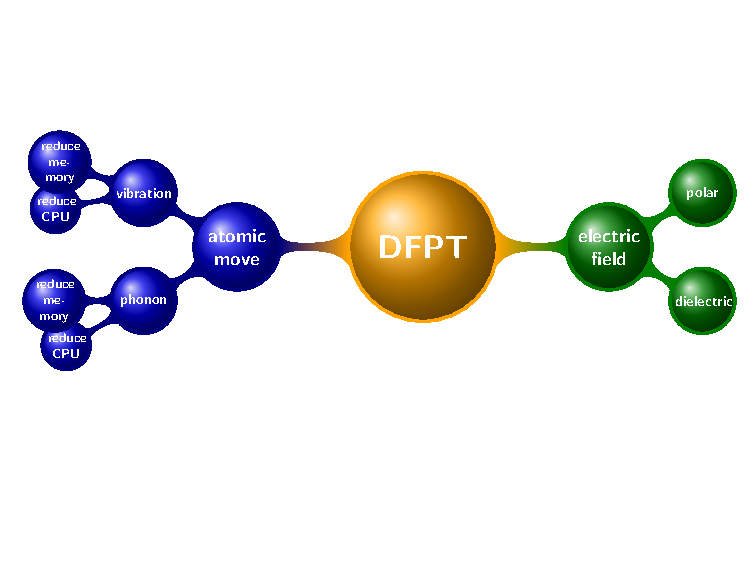
\includegraphics[width=0.98\columnwidth]{DFPT_map}
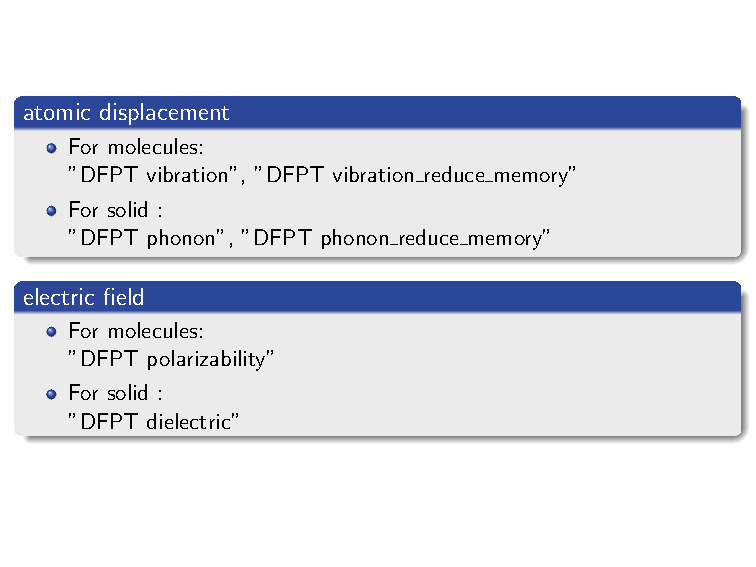
\includegraphics[width=0.98\columnwidth]{DFPT_toolkit}
\caption{The DFPT feathers in FHI-aims.}
\end{figure}





\subsection*{Theory}
\subsubsection{Lattice Dynamics}
In order to get vibration/phonon frequencies, first we need to get dynamical matrix, 
Let's define a lattice vector $\mathbf{R}_{Im}$ as 
\begin{equation}
\mathbf{R}_{Im} = \mathbf{R}_I+\mathbf{R}_m,
\label{PeriodicImage}
\end{equation}
whereby $\mathbf{R}_m$ denotes an arbitrary linear combination of~$\mathbf{a}_1$, $\mathbf{a}_2$, and $\mathbf{a}_3$. 
And the dynamical matrix $D_{IJ}(\mathbf{q})$ is a Fourier transform of harmonic Hessian matrix (Force constant) $\Phi_{Im,J}^{harm}$. 
\begin{align}
D_{IJ}(\mathbf{q}) &=\dfrac{1}{\sqrt{M_I M_J}} \sum_{m} \Phi_{Im,J}^{harm} \exp{\left(i\mathbf{q}\cdot\mathbf{R_m}\right)}  \nonumber \\
&=\dfrac{1}{\sqrt{M_I M_J}} \sum_{m}\dfrac{d^2 E_{KS}}{d \mathbf{R}_{Im} d \mathbf{R}_{J}  }\exp{\left(i\mathbf{q}\cdot\mathbf{R_m}\right)} 
\label{dynmat_FT}
\end{align}

Since the finite~($3N\times 3N$) dynamical matrix~$\mathbf{D}(\mathbf{q})$ would in principle have to be determined for an infinite number of $\mathbf{q}$-points in the Brillouin zone.  Its diagonalization would produce a set of $3N$ $\mathbf{q}$-dependent eigenfrequencies~$\omega_\lambda(\mathbf{q})$ and -vectors~$\mathbf{e}_\lambda(\mathbf{q})$. 

In order to derive the second order derivatives for
total energy \textbf{analytically} (which is the key idea for the DFPT approach), the ground state total energy and force is derived first and we could get this second order derivatives directly. It is should be 
noted that, here real-space DFPT method is used,
so that we could get the real-space force constant
directly. 


In FHI-aims, the total energy is calculated by using band-energy, a derivation for cluster systems is a following, and the extending to extended systems is straightforward.
\[
E_{KS}=-\dfrac{1}{2}\sum_{i}<\phi_i|\nabla^2|\phi_i>-\int {n(\mathbf{r})  \sum_{I}\dfrac{Z_{I}}{|\mathbf{r}-\mathbf{R}_{I}|}  d\mathbf{r}}+
\]
\begin{equation}
 \dfrac{1}{2}\int \int {\dfrac{n(\mathbf{r}) n(\mathbf{r'}) }{|\mathbf{r}-\mathbf{r'} |}  d\mathbf{r}  d\mathbf{r'}} +\dfrac{1}{2}\sum_{I}\sum_{J\neq I}{\dfrac{Z_{I} Z_{J}}{|\mathbf{R}_{I}-\mathbf{R}_{J} |} }+ E_{xc}(n)
 \label{eq:E_KS_original}
\end{equation}
using 
\[
\Rightarrow
\hat{h_{ks}}=-\dfrac{1}{2}\nabla^2- \sum_{I}\dfrac{Z_{I}}{|\mathbf{r}-\mathbf{R}_{I}|}
+ \int {\dfrac{n(\mathbf{r'}) }{|\mathbf{r}-\mathbf{r'} |}  d\mathbf{r'}} + v_{xc}(\mathbf{r})
\]
we have 
\[
= \sum_{i}<\phi_i|\hat{h_{ks}}|\phi_i> -\int{[n(\mathbf{r}) v_{xc}(\mathbf{r})] d\mathbf{r}} +E_{xc}(n)
\]
\begin{equation}
-\dfrac{1}{2}\int \int {\dfrac{n(\mathbf{r}) n(\mathbf{r'}) }{|\mathbf{r}-\mathbf{r'} |}  d\mathbf{r}  d\mathbf{r'}} 
+\dfrac{1}{2}\sum_{I}\sum_{J\neq I}{\dfrac{Z_{I} Z_{J}}{|\mathbf{u}_{I}-\mathbf{u}_{I} |} }
\end{equation}
\[
=\sum_{i}{f_i \epsilon_{i}}-\int{[n(\mathbf{r}) v_{xc}(\mathbf{r})] d\mathbf{r}} +E_{xc}(n)
\]
\begin{equation}
-\dfrac{1}{2}\int \int {\dfrac{n\mathbf{r}) n(\mathbf{r'}) }{|\mathbf{r}-\mathbf{r'} |}  d\mathbf{r}  d\mathbf{r'}} 
+\dfrac{1}{2}\sum_{I}\sum_{J\neq I}{\dfrac{Z_{I} Z_{J}}{|\mathbf{R}_{I}-\mathbf{R}_{I} |} }
\end{equation}

\[
=\sum_{i}{f_i \epsilon_{i}}-\int{[n(\mathbf{r}) v_{xc}(\mathbf{r})] d\mathbf{r}} +E_{xc}(n)
\]
\[
-\dfrac{1}{2}\int \int {\dfrac{n(\mathbf{r}) n(\mathbf{r'}) }{|\mathbf{r}-\mathbf{r'} |}  d\mathbf{r}  d\mathbf{r'}} 
+\dfrac{1}{2}\int {n(\mathbf{r})  \sum_{I}\dfrac{Z_{I}}{|\mathbf{r}-\mathbf{R}_{I}|}  d\mathbf{r}}
\]
\begin{equation}
+\dfrac{1}{2}\sum_{I}\sum_{J\neq I}{\dfrac{Z_{I} Z_{J}}{|\mathbf{R}_{I}-\mathbf{R}_{J} |} }
-\dfrac{1}{2}\int {n(\mathbf{r})  \sum_{I}\dfrac{Z_{I}}{|\mathbf{r}-\mathbf{R}_{I}|}  d\mathbf{r} }
\end{equation}
\[
=\sum_{i}{f_i \epsilon_{i}}-\int{[n(\mathbf{r}) v_{xc}(\mathbf{r})] d\mathbf{r}} +E_{xc}(n)
\]
\[
-\dfrac{1}{2}\int n(\mathbf{r}) [\sum_{I} V^{free}_I(|\mathbf{r}-\mathbf{R}_I|)+\delta V_I(|\mathbf{r}-\mathbf{R}_I|) ]   d\mathbf{r}
\]
\begin{equation}
-\dfrac{1}{2}\sum_{I}Z_{I} [\sum_{J} V^{free}_J(|\mathbf{R}_J-\mathbf{R}_I|)+\sum_{J\ne I}\delta V_J(|\mathbf{R}_J-\mathbf{R}_I|) ]  
\end{equation}
\[
=\sum_{i}{f_i \epsilon_{i}}-\int{[n(\mathbf{r}) v_{xc}(\mathbf{r})] d\mathbf{r}} +E_{xc}(n)
\]
\[
-\dfrac{1}{2}\int n(\mathbf{r}) [\sum_{I} V^{es,tot}_I(|\mathbf{r}-\mathbf{R}_I|)]   d\mathbf{r}
\]
\begin{equation}
-\dfrac{1}{2}\sum_{I}Z_{I} [V^{es,tot}_I(0)+\sum_{J\ne I} V^{es,tot}_J(|\mathbf{R}_J-\mathbf{R}_I|) ]  
\label{eq:E_KS_new-functional}
\end{equation}
Here Eq.(\ref{eq:E_KS_new-functional}) is exactly the one to calculate Kohn-Sham total energy. An 
extension expression to extended system is in Eq.\ref{eq:E_KS_uc_new-functional-PBC}
\begin{eqnarray}
\label{eq:E_KS_uc_new-functional-PBC}
E_{tot}=-\dfrac{1}{N_k}\sum_{i}^{uc}{f_{\mathbf{k}i} \epsilon_{\mathbf{k}i}}-\int_{uc}{[n(\mathbf{r}) v_{xc}(\mathbf{r})] d\mathbf{r}} +E_{xc}(n) \\
-\dfrac{1}{2}\int_{uc} n(\mathbf{r}) [\sum_{I,m} V^{es,tot}_I(|\mathbf{r}-\mathbf{R}_{I,m}|)]   d\mathbf{r}   \nonumber \\
-\dfrac{1}{2}\sum_{I}Z_{I} [V^{es,tot}_I(0)+\sum_{(J,m)\ne (I,0)} V^{es,tot}_J(|\mathbf{R}_{Jm}-\mathbf{R}_{I}|) ]  \nonumber
\end{eqnarray}


Then we get the analytical force expression for cluster systems:
 \[
F_{I}= - \dfrac{d E_{KS}}{d\mathbf{R}_{I} } = \mathbf{F}_I^{HF} + \mathbf{F}_I^{P} + \mathbf{F}_I^{M}
\]
\[
-[ - \dfrac{\partial{(\int {n(\mathbf{r})  \sum_{I}\dfrac{Z_{I}}{|\mathbf{r}-\mathbf{R}_{I}|}  d\mathbf{r}})} }{ \partial{\mathbf{R}_{I}}} +
\dfrac{\partial{(\dfrac{1}{2}\sum_{I}\sum_{J\neq I}{\dfrac{Z_{I} Z_{J}}{|\mathbf{R}_{I}-\mathbf{R}_{J} |} })} }{\partial{\mathbf{R}_{I}}}  ]
\]
\[
-\sum_{\mu \nu}[ P_{\mu \nu}\int (\dfrac{\partial \chi_{\mu}}{\partial \mathbf{R}_{I} } \hat{h}_{ks} \chi_{\nu}   + \chi_{\mu} \hat{h}_{ks}  \dfrac{\partial \chi_{\nu}}{\partial \mathbf{R}_{I} } ) d\mathbf{r}    - W_{\mu\nu} \dfrac{\partial S_{\mu \nu}}{\partial \mathbf{R}_{I} } ]
\]
\begin{equation}
-\int{[n(\mathbf{r})-n^{MP}(\mathbf{r})] \dfrac{\partial{ V^{MP}(\mathbf{r})} }
{\partial{\mathbf{R}_{I}} } d\mathbf{r} 
}
\label{eq:force}
\end{equation}

Here $P_{\mu \nu}$ refers to density matrix and 
$W_{\mu \nu}$  refers to energy density matrix. 
Here the first term is Hellmann-Feynman force using Hellmann-Feynman theorem ; The second term is Pulay term, it comes from basis set dependence of atomic coordinate; The third term is multipole force, it count the contribution from multipole expansion error for Hartree energy calculation (multipole Poisson solver).


Under periodic boundary conditions, we get the following expression for force for extended systems: 
\begin{equation}
\mathbf{F}_J^{HF}= Z_{J}[\dfrac{\partial V^{es,tot}_{J}(0)} {\partial \mathbf{R}_{J} } +  \sum_{(I,m)\ne(J,0)}(
\dfrac{\partial V^{es,tot}_{I}(|\mathbf{R}_{J}-\mathbf{R}_{Im}) |} {\partial \mathbf{R}_{J} }  )  ]
\label{eq:F_HF_PBC} 
\end{equation}
\begin{align}
\mathbf{F}_J^{P} = - \dfrac{2}{N_k}\sum_{\mathbf{k},i,\mu,\nu}\int {f_{i\mathbf{k}}C^{*}_{\mu i\mathbf{k}}\dfrac{\partial \varphi_{\mu\mathbf{k}}^{*}(\mathbf{r})}{\partial  \mathbf{R}_{J} }(\hat{h}_{ks}-\epsilon_{i\mathbf{k}}) C_{\nu i\mathbf{k}}\varphi_{\nu\mathbf{k}}(\mathbf{r}) d\mathbf{r} }   \;,
\label{eq:F_pulay_PBC} 
\end{align}


In our real-space DFPT method, this harmonic Hessian matrix is calculated directly, as explained in our paper. 
The Hessian can be split into  two part

\begin{equation}
E_{KS}^{(2)}=\dfrac{d^2{E_{KS}} }{d{\mathbf{R}_{I}} d{\mathbf{R}_{J}}}=\Phi_{I,J}^{HF} + \Phi_{I,J}^{P} + Phi_{I,J}^{MP}
\label{eq:Hessian_KS}
\end{equation}
\[
=[ - \dfrac{\partial^{2} {(\int {n(\mathbf{r})  \sum_{I}\dfrac{Z_{I}}{|\mathbf{r}-\mathbf{R}_{I}|}  d\mathbf{r}})} }{ \partial{\mathbf{R}_{I}}\partial{\mathbf{u}_{J}}} +
\dfrac{\partial^{2}{(\dfrac{1}{2}\sum_{I}\sum_{J\neq I}{\dfrac{Z_{I} Z_{J}}{|\mathbf{R}_{I}-\mathbf{R}_{J} |} })} }{\partial{\mathbf{R}_{I}} \partial{\mathbf{R}_{J}}}  ]
\]

\[
+\sum_{\mu\nu}{ \dfrac{\partial  P_{\mu\nu}}{\partial {\mathbf{R}_{J} } }\int( \dfrac{\partial \chi_{\mu}}{\partial \mathbf{R}_{I}} \hat{h}_{ks} \chi_{\nu} +  \chi_{\mu}\hat{h}_{ks}\dfrac{\partial \chi_{\nu}}{\partial \mathbf{R}_{I}} ) d\mathbf{r} }
\]
\[
 + \sum_{\mu\nu}P_{\mu\nu}\int [\dfrac{\partial^2 \chi_{\mu}}{\partial \mathbf{R}_I \partial \mathbf{R}_J} \hat{h}_{ks} \chi_{\nu}  
 + \dfrac{\partial \chi_{\mu}}{\partial \mathbf{R}_I } \dfrac{\partial \hat{h}_{ks} }{\partial \mathbf{R}_J}  \chi_{\nu}
 + \dfrac{\partial \chi_{\mu}}{\partial \mathbf{R}_I } \hat{h}_{ks}  \dfrac{\partial \chi_{\nu}}{\partial \mathbf{R}_J}  ]  d\mathbf{r} 
\]
\[ 
+\sum_{\mu\nu}P_{\mu\nu}\int [  
\dfrac{\partial \chi_{\mu}}{\partial \mathbf{R}_J } \hat{h}_{ks} \dfrac{\partial \chi_{\nu}}{\partial \mathbf{R}_I}  + \chi_{\mu} \dfrac{\partial \hat{h}_{ks}}{\partial \mathbf{R}_J} \dfrac{\partial \chi_{\nu}}{\partial \mathbf{R}_I }
+\chi_{\nu} \hat{h}_{ks}\dfrac{ \partial^2 \chi_{\nu}}{\partial \mathbf{R}_I \partial \mathbf{R}_J}  ]  d \mathbf{r}   
\]
\[ 
-(\sum_{\mu\nu}{ \dfrac{\partial E_{ \mu\nu}}{\partial \mathbf{R}_J }     \dfrac{\partial S_{ \mu\nu}}{\partial \mathbf{R}_I }      }+ \sum_{\mu\nu}{E_{\mu\nu} \dfrac{ \partial^2 S_{\mu\nu}}{\partial \mathbf{R}_I \partial \mathbf{R}_J} } )      
\]
\[
+\int{\dfrac{\partial [n(\mathbf{r})-n^{MP}(\mathbf{r})]}{ \partial \mathbf{R}_I} \dfrac{\partial V^{MP}(\mathbf{r})}{\partial \mathbf{R}_J } d\mathbf{r} } 
\]
\[
+\int{[n(r)-n^{MP}(r)] \dfrac{\partial^2  V^{MP}(r)}{\partial \mathbf{R}_I \partial\mathbf{R}_J} d\mathbf{r} } 
\]

It can also be divided into three part: Hellmann-Feynman Hessian,
Pulay Hessian, Multipole Hessian. In real calculation, we
drop multipole Hessian due to its value is only $10^{-3}$ times small
compared with the other two. 

Under periodic boundary conditions, we get the following expression for force constants:
\begin{equation}
\Phi^{harm}_{Is,J}= \frac{d^2\mathbf{E}^{KS}}{d\mathbf{R}_{Is}d\mathbf{R}_{J}} 
=- \frac{d\mathbf{F}_{J}}{d\mathbf{R}_{Is}}
=- \frac{d\mathbf{F}_{Is}}{d\mathbf{R}_{J}} 
=\Phi_{Is,J}^{HF} + \Phi_{Is,J}^{P}  \;.
\end{equation}

\begin{eqnarray}
\Phi_{Is,J}^{HF} & = & -Z_{J}\left(\frac{d}{d\mathbf{R}_J}\dfrac{\partial V^{es}_{J}(0)} {\partial \mathbf{R}_{J} }\right) \delta_{Is,J0}\\ && - Z_J\left(\dfrac{d}{d\mathbf{R}_{J}} \dfrac{\partial V^{es,tot}_{I}(|\mathbf{R}_{J}-\mathbf{R}_{Is}) |} {\partial \mathbf{R}_{Is} }  \right) \left(1-\delta_{Is,J0}\right)\;,\nonumber
\end{eqnarray}
in which $\delta_{Is,J0} = \delta_{IJ}\delta_{s0}$ denotes
a multi-index Kronecker delta. 

For the sake of readability, its total derivative is split into four terms:
\begin{equation}
\Phi_{Is,J}^{P} = \Phi_{Is,J}^{P-P} + \Phi_{Is,J}^{P-H} + \Phi_{Is,J}^{P-W} + \Phi_{Is,J}^{P-S}\;.
\end{equation}


The first term
\begin{equation}
\Phi_{Is,J}^{P-P} =  {2} \sum_{\mu m,\nu n} 
\left( \frac{d P_{\mu m,\nu n}}{d \mathbf{R}_{J}}\right)
\int  \dfrac{\partial \chi_{\mu m}(\mathbf{r})}{\partial  \mathbf{R}_{Is} }\hat{h}_{ks} \chi_{\nu n}(\mathbf{r}) \, d\mathbf{r}
\end{equation}

accounts for the response of the density matrix~$P_{\mu m,\nu n}^{m,n}$. The second term 
\begin{eqnarray}
\Phi_{Is,J}^{P-H} & = &  
2\sum_{\mu m,\nu n}  
P_{\mu m,\nu n} \cdot\\ 
&&\left(
\int  \dfrac{\partial^2 \chi_{\mu m}(\mathbf{r})}{\partial  \mathbf{R}_{Is}\partial  \mathbf{R}_{J} }\,\hat{h}_{ks}\, \chi_{\nu n}(\mathbf{r}) \, d\mathbf{r}\right.\\
&&+\int  \dfrac{\partial \chi_{\mu m}(\mathbf{r})}{\partial  \mathbf{R}_{Is} }\frac{d \hat{h}_{ks}}{d\mathbf{R}_{J}}\chi_{\nu n}(\mathbf{r}) \, d\mathbf{r}\\
&&\left.+\int  \dfrac{\partial \chi_{\mu m}(\mathbf{r})}{\partial  \mathbf{R}_{Is} }\hat{h}_{ks}\frac{\partial \chi_{\nu n}(\mathbf{r})}{\partial \mathbf{R}_{J}} \, d\mathbf{r}
\right)
\end{eqnarray}
accounts for the response of the Hamiltonian~$\hat{h}_{ks}(\mathbf{k})$, while the third  and fourth term
\begin{eqnarray}
\Phi_{Is,J}^{P-W} & = &  - 2\sum_{\mu m,\nu n }
\frac{d W_{\mu m,\nu n}}{d\mathbf{R}_{J}}
\int  \dfrac{\partial \chi_{\mu m}(\mathbf{r})}{\partial  \mathbf{R}_{Is} }\chi_{\nu n}(\mathbf{r}) \, d\mathbf{r}
\label{PhiPW}\\
\Phi_{Is,J}^{P-S} & = &  - 2\sum_{\mu m,\nu n } 
W_{\mu m,\nu n} \dfrac{\partial}{\partial\mathbf{R}_{J} }
\int  \dfrac{\partial \chi_{\mu m}(\mathbf{r})}{\partial  \mathbf{R}_{Is} }\chi_{\nu n}(\mathbf{r}) \, d\mathbf{r} \label{PhiPS}
\end{eqnarray}
for the response of the energy weighted density matrix~$W_{\mu m,\nu n}$ and the overlap matrix~$S_{\mu m,\nu n}$, 
respectively, 
Please note that in all four contributions many terms vanish due to the fact that the localized atomic orbitals~$\chi_{\mu m}(\mathbf{r})$ are associated with one specific atom/periodic image~$\mathbf{R}_{J(\mu) m}$, which implies,~e.g.,
\begin{equation}
\frac{\partial \chi_{\mu m}(\mathbf{r})}{\partial \mathbf{R}_{Is}} = 
\frac{\partial \chi_{\mu m}(\mathbf{r})}{\partial \mathbf{R}_{Is}} \delta_{J(\mu)m,Is} \; .
\end{equation}

In in above force constants, it is clear that the first order density matrix $\dfrac{\partial  P_{\mu\nu}}{\partial {\mathbf{R}_{J} }}$ and the 
first order energy density matrix $\dfrac{\partial  W_{\mu\nu}}{\partial {\mathbf{R}_{J} }}$ are needed. These first order qualtities are obtained in the DFPT cycle. The flowchart of our DFPT
cycle for lattice dynamics is shown in Fig.\ref{fig:DFPT_lattice_dynamics_flowchart}.

\begin{figure}
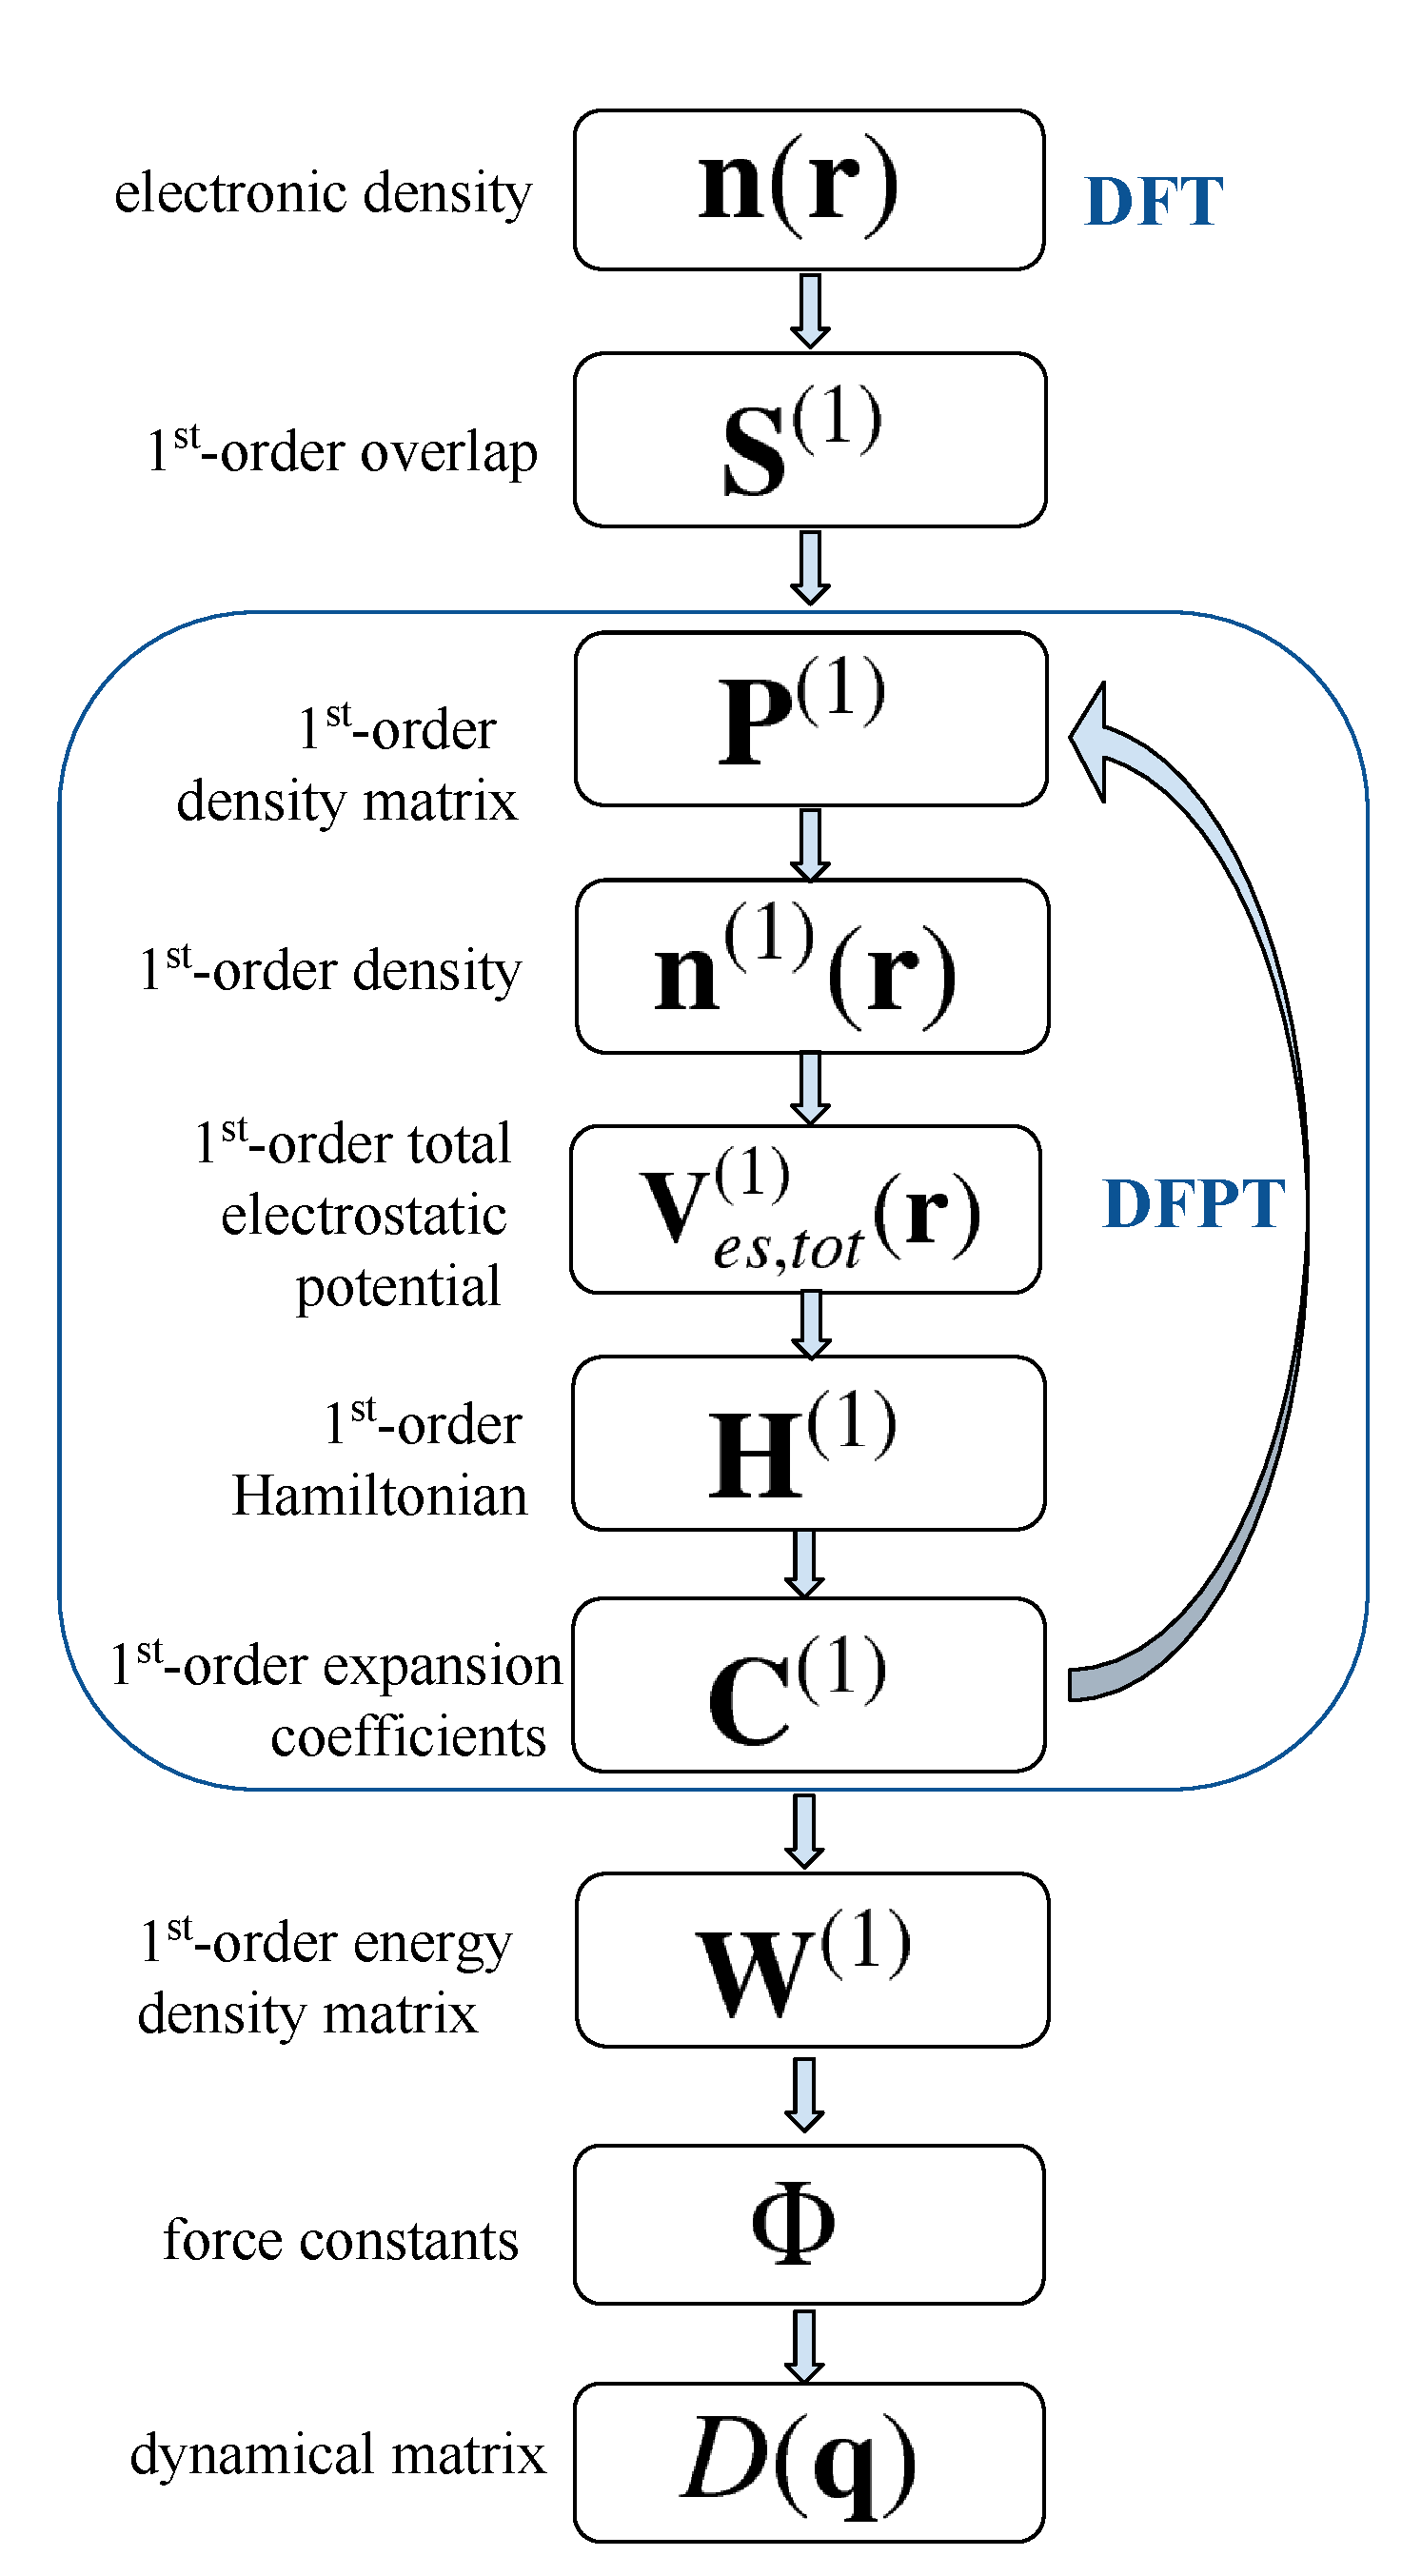
\includegraphics[width=0.7\columnwidth]{DFPT_lattice_dynamics_flowchart}
\caption{Flowchart of the lattice dynamics implementation using a real-space DFPT formalism.}
\label{fig:DFPT_lattice_dynamics_flowchart}
\end{figure}




Our resulting frequencies look like this:
{\footnotesize
\begin{verbatim}
DFPT-Results:

List of all frequencies found:
  Mode number      Frequency [cm^(-1)]   IR-intensity [D^2/Ang^2]
            1           -2282.47061452                 0.00000000
            2           -2282.47061452                 0.00000000
            3              -0.00004008                 0.00000001
            4               0.00003217                 0.00000000
            5               0.00006390                 0.00000000
            6            5546.30603353                 0.00000000
\end{verbatim}
}


For vibration calculation, there are there keywords to choose:
\begin{itemize}
\item DFPT vibration 
\item DFPT vibration\_reduce\_memory
\item DFPT vibration\_with\_moving\_grid\_effect
\end{itemize}
A comparison for these three features as well as DFT calculation is shown in Fig.\ref{fig:DFPT_compare}



\begin{figure}
\includegraphics[width=1.0\columnwidth]{DFPT_compare}
\caption{The memory profiles using valgrind are shown for DFT and three DFPT vibration keywords.    It is clearly shown that the DFPT\_vibration\_reduce\_memory(28.4 MB) code just use nearly the same memory as DFT (28.0MB) calculation, while DFPT\_vibration(33.2 MB) and DFPT\_vibration\_with\_moving\_gird(34.6 MB) need higher memory because they stored matrix as
    (3,n\_atoms, *).  %DFPT\_vibration\_with\_moving\_gird(34.6 MB) is higher than DFPT\_vibration(33.2 MB) because it has additional
% partition\_deriv\_delley(1:3,1:n\_atoms,1:n\_full_points) array.
%
%     About the CPU time, we can see that DFPT\_vibration\_with\_moving\_gird (169 s)  is also slower than DFPT\_vibration(161 s) as the
%     partition\_deriv\_delley(1:3,1:n\_atoms,1:n\_full\_points)  need to be calculated.
      }
\label{fig:DFPT_compare}
\end{figure}




In phonon calculation, only Gamma point results is printed in the output like this:
{\footnotesize
\begin{verbatim}
 =============================================
 DFPT-Results: for q1=  0.000000000000000E+000  0.000000000000000E+000
  0.000000000000000E+000
 =============================================

 List of all frequencies found:
  Mode number      Frequency [cm^(-1)]
            1           -2376.08047043
            2           -2376.08047043
            3              -0.00004497
            4               0.00001694
            5               0.00009141
            6            5113.49725256
\end{verbatim}
}

A typical phonon band structure is shown for Graphen in Fig. \ref{fig:graphen}

\begin{figure}
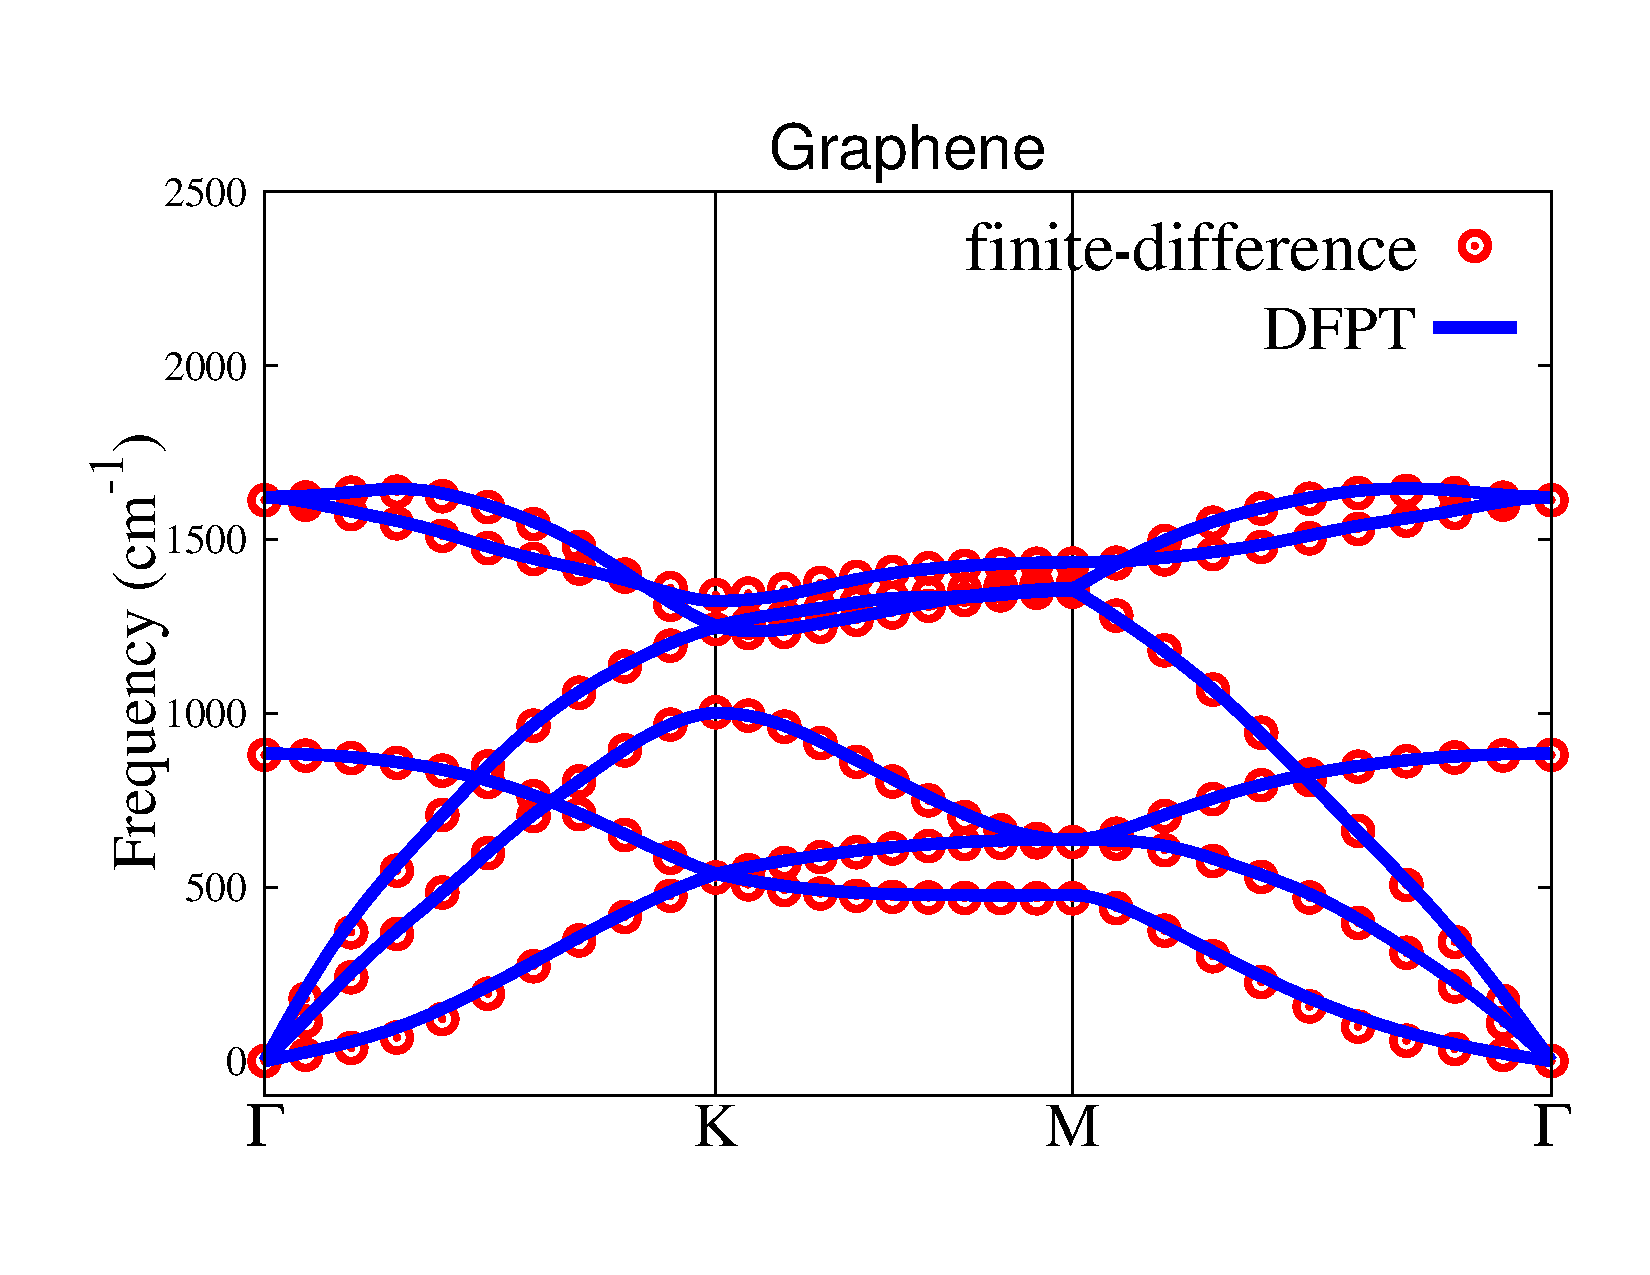
\includegraphics[width=1.0\columnwidth]{graphen_phonon_compare}
\caption{Vibrational band structure of graphene computed at the LDA level using
both DFPT~(solid blue line) and finite differences~(red open circles). All calculations
have been performed using a 11$\times$11$\times$1 $\mathbf{k}$-grid sampling for the 
primitive Brillouin zone, tight settings for the
integration, and a tier 1 basis set.}
\label{fig:graphen}
\end{figure}

A scaling test for DFPT code for lattice dynamics is has been done for Si system, with up to 1024 atoms in the unit cell see Fig.\ref{fig:scaling_Si}.
\begin{figure}
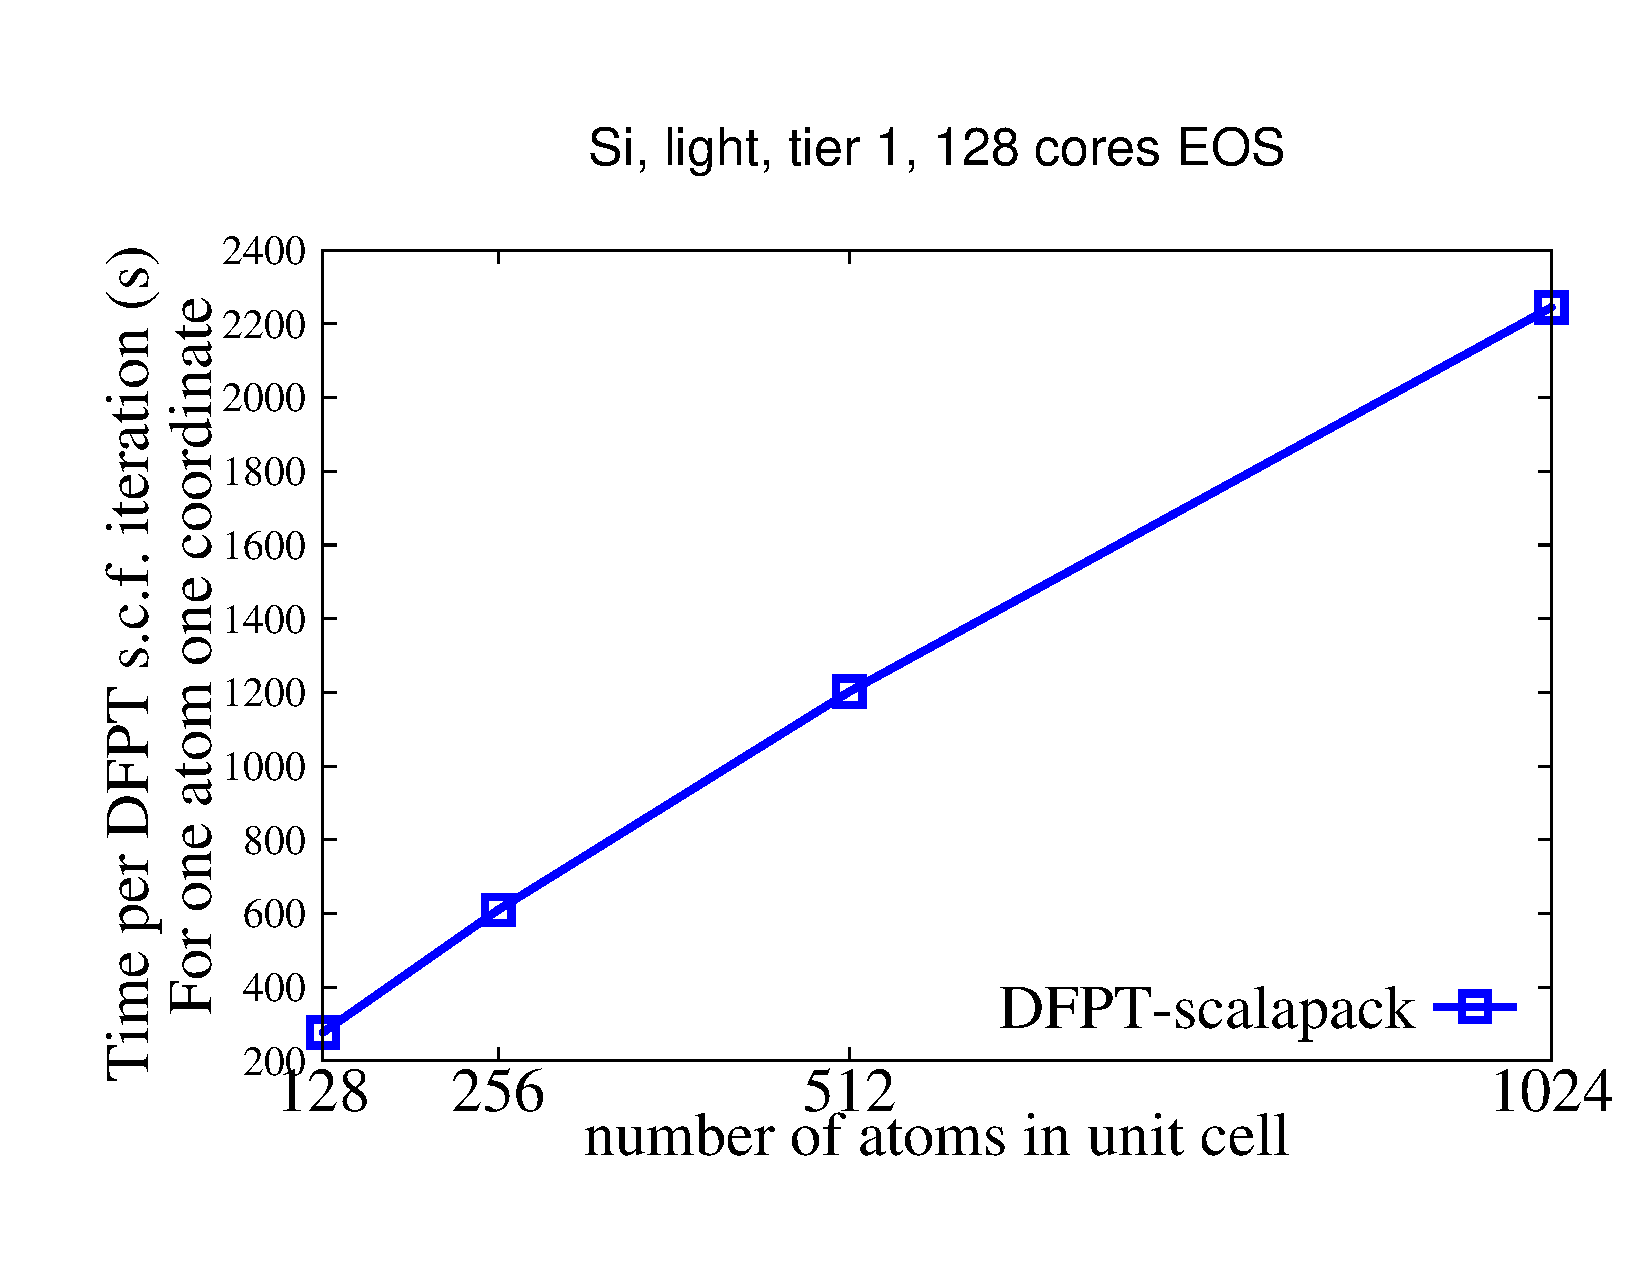
\includegraphics[width=1.0\columnwidth]{DFPT_scaling_Si}
\caption{The CPUT time per DFPT cycle as a function of the number of atoms in unit cell on 128 CPU cores.}
\label{fig:scaling_Si}
\end{figure}





\subsubsection{Homogeneous Electric Fields}
Suppose we have an external electrical field $\mathbf{\xi }$, the Hamitonian is changed by adding the following term:
\begin{equation}
H_{E}=- \mathbf{r} \cdot \mathbf{\xi}
\end{equation}
and the induced total energy becomes: 
\begin{equation}
E_{tot}=E^0_{tot} - \sum_{I=x,y,z}\mu_{I}\xi_{I}-
\dfrac{1}{2}\sum_{I,J}\alpha_{I J}\xi_{I}\xi_{J}
\end{equation}
Here $\mu_{I}$ label the dipole moment, 
\begin{equation}
\mu_{I}=\int{n(\mathbf{r}) r_I d\mathbf{r} }
\end{equation}
and the corresponding polarizability is defined as the first order derivative of dipole moment with respect to external electrical field :
\begin{equation}
\alpha_{I,J}= \dfrac{\partial \mu_{I}}{\partial \xi_{J}}= \int{ r_I \dfrac{\partial n(\mathbf{r})}{\partial \xi_{J} } d \mathbf{r}}
\label{eq:polar}
\end{equation}
The polarizability for cluster system can be calculated using \ref{eq:polar} without any problem. However, for extended systems, the position operator is 
unbound, in order to deal with it, we use 
$
\braket{\psi_{i}(\mathbf{k})|-\mathbf{r}|\psi_{j}(\mathbf{k})}=\dfrac{\braket{\psi_{i}(\mathbf{k})|\mathbf{\bigtriangledown}|\psi_{j}(\mathbf{k})}}{(\varepsilon_i(\mathbf{k})-\varepsilon_j(\mathbf{k}))}
$
, so we can rewritten polarizability (Eq.{\ref{eq:polar}) for extended system as
\begin{align}
\alpha_{I,J}& = \int_{uc}{r_I \dfrac{\partial n(\mathbf{r})}{\partial \xi_{J} }  d \mathbf{r}} \\
%     & = \dfrac{4}{N_k} \int_{uc}{r_I \sum_{i,\mathbf{k}} \left( \dfrac{\partial \psi_{i}(\mathbf{k})}{\partial \xi_{J} }\right) \psi^{*}_{i}(\mathbf{k})   d \mathbf{r}} \\ 
%     & =  \dfrac{4}{N_k} \int_{uc}{r_I \sum_{i,\mathbf{k}} \left( \sum_{j}\psi_{j}(\mathbf{k})
%   \dfrac{\braket{\psi_j(\mathbf{k})| H^{(1)}|\psi_i(\mathbf{k})}_{uc}}{\varepsilon_i(\mathbf{k})-\varepsilon_j(\mathbf{k})} \right)  \psi^{*}_{i}(\mathbf{k})   d \mathbf{r}} \\ 
%   & =  \dfrac{4}{N_k} \sum_{i,j,\mathbf{k}}\braket{\psi_i(\mathbf{k})|r_I|\psi_j(\mathbf{k})}_{uc} \dfrac{\braket{\psi_j(\mathbf{k})| H^{(1)}|\psi_i(\mathbf{k})}_{uc}}{\varepsilon_i(\mathbf{k})-\varepsilon_j(\mathbf{k})} \\
  & =\dfrac{4}{N_k} \sum_{i,j,\mathbf{k}}\braket{\psi_i(\mathbf{k})|\nabla_I|\psi_j(\mathbf{k})}_{uc} \dfrac{\braket{\psi_j(\mathbf{k})| H^{(1)}|\psi_i(\mathbf{k})}_{uc}}{(\varepsilon_j(\mathbf{k})-\varepsilon_i(\mathbf{k}))^2}
\end{align}
and the corresponding dielectric constant is 
\begin{equation}
\epsilon_{IJ}^{\infty}=\delta_{IJ} + \dfrac{4\pi}{V_{uc}} \alpha_{IJ}
\end{equation}

Similar to the lattice dynamic case, the first order density matrix $\dfrac{\partial  P_{\mu\nu}}{\partial {\mathbf{R}_{J} }}$ is needed to be calculated using DFPT cycles. The flowchart of our DFPT
cycle for electric field is shown in Fig.\ref{fig:DFPT_E_field_flowchart}.

\begin{figure}
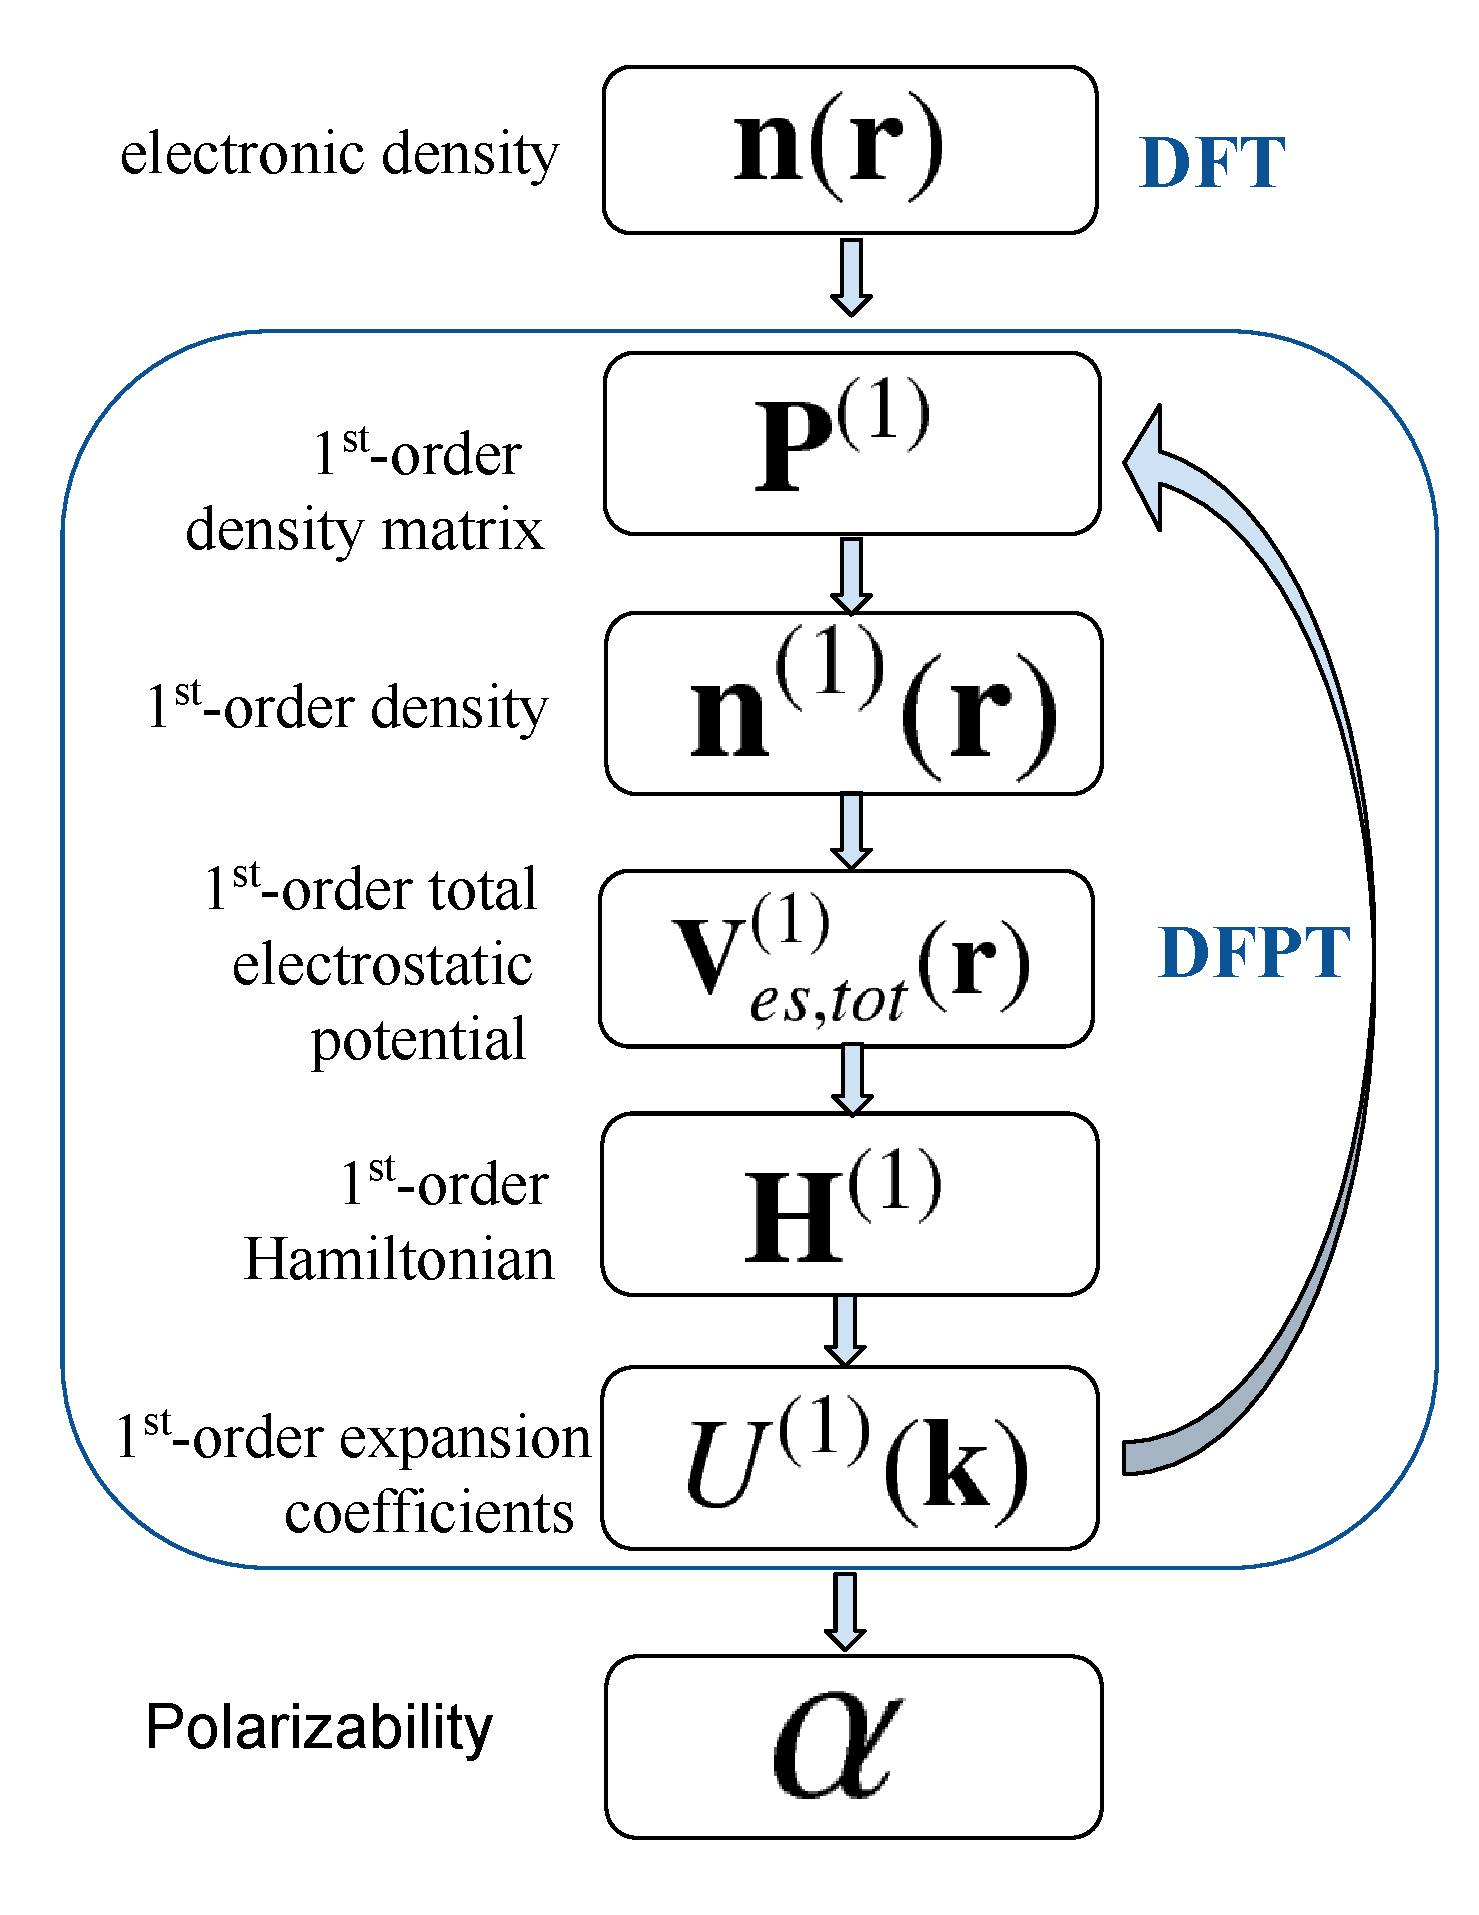
\includegraphics[width=0.7\columnwidth]{DFPT_flowchart_E_filed}
\caption{Flowchart of the electric field implementation using a real-space DFPT formalism.}
\label{fig:DFPT_E_filed_flowchart}
\end{figure}


In order to validate our implementation for extended system,
we compare the polarisability with cluster extended method,
We use hydrogen line (H$_2$) as a showcase. All calculations have been performed with a geometry shown in Fig.\ref{fig:H2_line} using the tight integration grids and "minimal" basis sets. For the periodic chain, a reciprocal-space
grid of $35 \times 1 \times 1$ electronic $\mathbf{k}$-points (in the primitive Brillouin zone) has been utilized as substantiated convergence in Tab.~\ref{tab:k_convergence_for_H2_line}. The convergence with respect to electronic $\mathbf{k}$-points is reasonably fast, in which k grid $35 \times 1 \times 1$ has already get converged with absolute 
and relative errors of $0.09$~Bohr$^{3}$ and $0.07$~\% compared with k grid $70 \times 1 \times 1$. 

\begin{table}
\begin{tabular}{c|c c c cc }
\hline \hline
k & 10 & 20 & 35 &  40 & 70 \\
\hline
$\alpha_{xx}$  & 180.49 & 134.76  &  130.17 & 130.29 & 130.26\\
\hline \hline
\end{tabular}
\caption{The $\mathbf{k}$-convergence tes for polarizabllities per H$_2$ unit cell.}
\label{tab:k_convergence_for_H2_line}
\end{table}

For cluster extended method, the results are fitted with an equation
\begin{equation}
\ln{(\alpha_N-\alpha_{N-1})}=a+\dfrac{b}{N}
\end{equation}
So the limiting value of the polarizability per unit cell with N going to infinity is given :
\begin{equation}
\lim_{N\rightarrow \infty}{\alpha_{uc}} = \exp(a)
\end{equation}
Here we fit the  DFPT results (N=52 to 64) with an equation
\begin{equation}
\ln{(\alpha_N-\alpha_{N-1})}=a+\dfrac{b}{N}
\end{equation}
So the limiting value of the polarizability per unit cell with N going to infinity is given :
\begin{equation}
\lim_{N\rightarrow \infty}{\alpha_{uc}} = \exp^{a}
\end{equation}
and finally get 
\begin{align}
a=4.857 \\
b=-1.123 \\
\end{align}
so we have $\alpha$(Extrapolation)$_{uc}=128.718$

%-------my python fitting code------------
%import numpy as np
%import matplotlib.pyplot as plt
%data=np.loadtxt('/home/shang/shanghui_like/my_little_plot/02_for_electric_field/H2_chain.dat')
%x=data[25:,0]
%y=data[25:,4]
%np.polyfit(1.0/x,np.log(y),1)
%#Polynomial coefficients, highest power first : so is x^2--x^1---x^0
%#x=array([ 52.,  54.,  56.,  58.,  60.,  62.,  64.])
%np.exp(4.85762699) = 128.7183893773757
%-------end my python fitting code---------

\begin{table}
\begin{tabular}{c|  c c}
\hline \hline
H$_{N}$ (a.u.)  &  $\alpha^{DFPT}_{N}$   & $\alpha^{DFPT}_{uc}$   \\
\hline
2    &  9.923  &  9.923 \\           
4    &  34.042  &  24.118 \\
6    &  73.134  &  39.092 \\
8    &  126.619  &  53.485 \\
10    &  193.231  &  66.612 \\
12    &  271.317  &  78.086 \\
14    &  359.107  &  87.790 \\
16    &  454.896  &  95.789 \\
18    &  557.150  &  102.254 \\
20    &  664.553  &  107.404 \\
22    &  776.018  &  111.464 \\
24    &  890.662  &  114.644 \\
26    &  1007.790  &  117.128 \\
28    &  1126.853  &  119.064 \\
30    &  1247.430  &  120.577 \\
32    &  1369.190  &  121.760 \\
34    &  1491.883  &  122.693 \\
36    &  1615.312  &  123.429 \\
38    &  1739.328  &  124.016 \\
40    &  1863.812  &  124.485 \\
42    &  1988.677  &  124.865 \\
44    &  2113.848  &  125.171 \\
46    &  2239.272  &  125.423 \\
48    &  2364.903  &  125.631 \\
50    &  2490.709  &  125.806 \\
52    &  2616.657  &  125.949 \\
54    &  2742.728  &  126.071 \\
56    &  2868.902  &  126.174 \\
58    &  2995.166  &  126.264 \\
60    &  3121.505  &  126.339 \\
62    &  3247.909  &  126.404 \\
64    &  3374.371  &  126.462 \\
\hline \hline
\end{tabular}
\caption{Total longitudinal polarizabllities calculated using PZ-LDA molecular hydrogen chains, with bond length alternation scheme A (H-H = 2.0 a.u., H$_2$-H$_2$ = 4.5 a.u. Also we list the longitudinal polarizabllities per H$_2$ unit cell calculated by $(\alpha_N-\alpha_{N-1})$. }
\end{table}



\begin{figure}
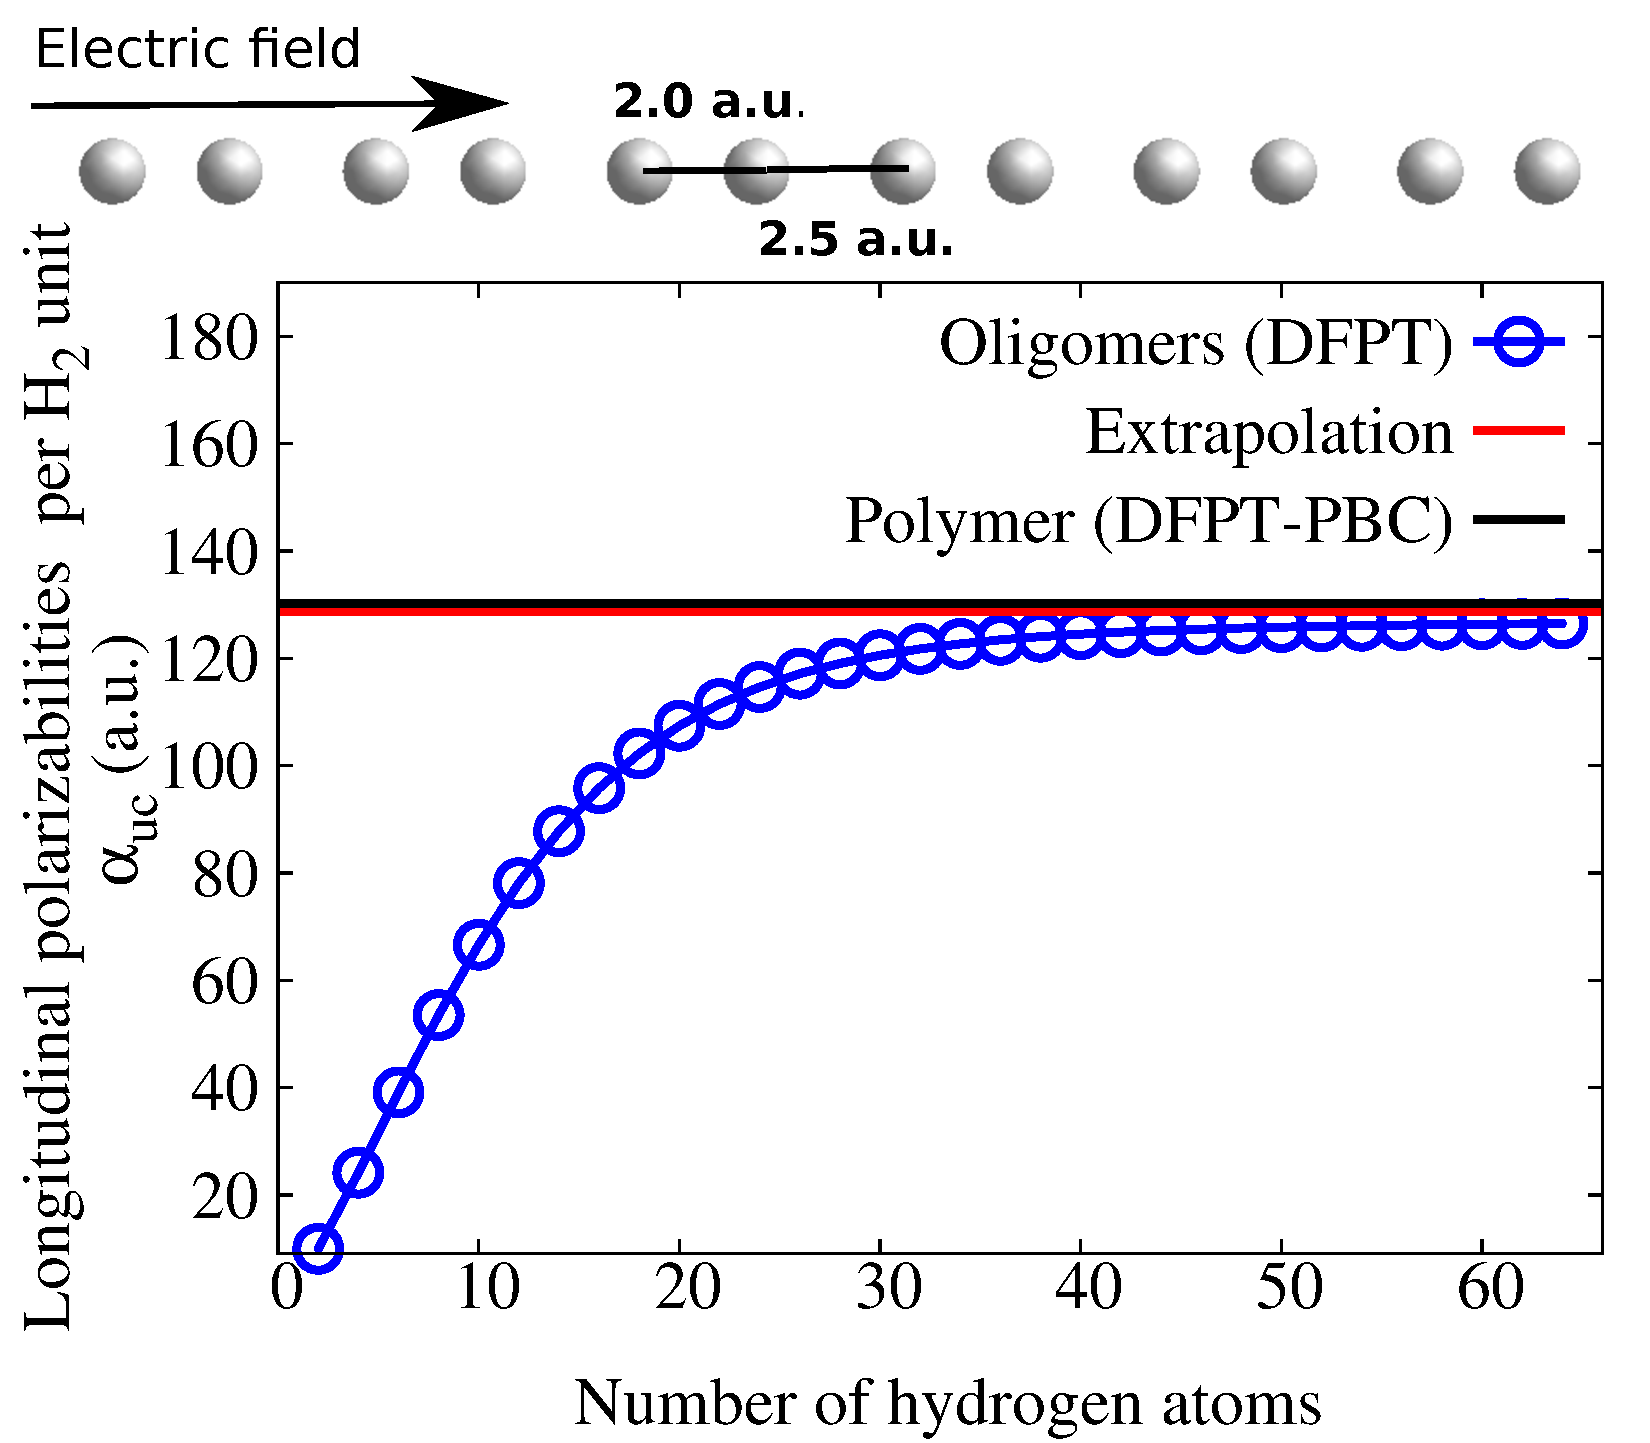
\includegraphics[width=0.9\columnwidth]{H2_chain_Extrapolation_PZ-LDA.pdf}
\caption{Total longitudinal polarizabllities per H$_2$ unit cell calculated using DFPT with PZ-LDA for molecular hydrogen chains, the bond length is H-H = 2.0 a.u., H$_2$-H$_2$ = 4.5 a.u., as shown in the figure. The extrapolated value of $\alpha^{DFPT}_{uc}$ is 128.7, listed with red line. The DFPT-PBC value is 130.2, listed with black line. }
\label{fig:H2_line}
\end{figure}



\subsection*{Some Technical details}
\subsubsection{Screened Method}
In periodic systems, the Coulomb potential is long range, e.g. in a H atom as shown in Fig. \ref{fig:combied }, both $V_{electron-ion}$
and $V^{free}_{electron-electron}$ are (separately) never zero (they decay as 1/$r$ but the number of atoms which they interact with in a periodic system
grows as $r^2$ with distance). 
If we use the neutral free atom potential instead, the 
potential will approach zero at the radius where the electron charge integrates to exactly $-$1,
which is a finite radius determined by the confinement potential in FHI-aims.
\begin{figure}
 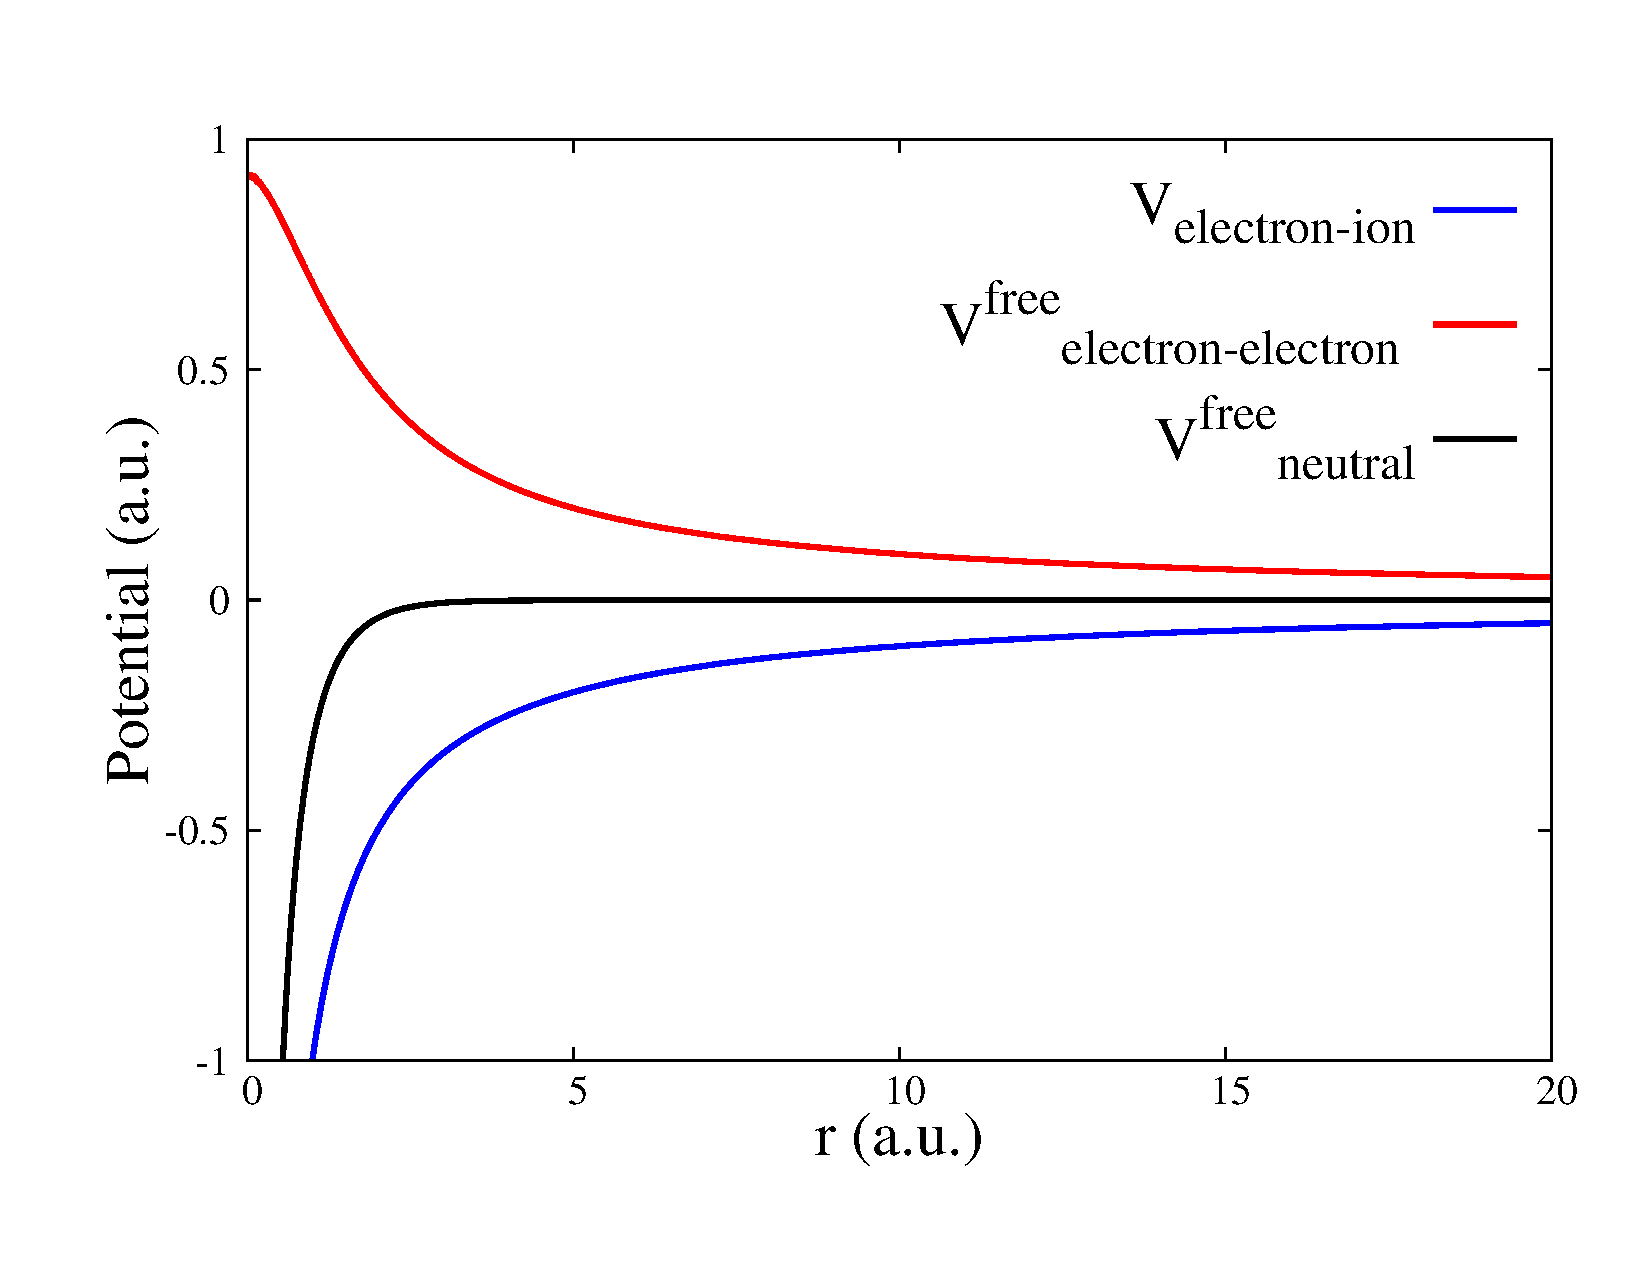
\includegraphics[width=0.7\columnwidth]{why_v_free}
 \caption{The screened scheme can remove long-range tail of Coulomb potential. Here we use H atom as an example.}
 \label{fig:combied }
\end{figure}
\begin{figure}
 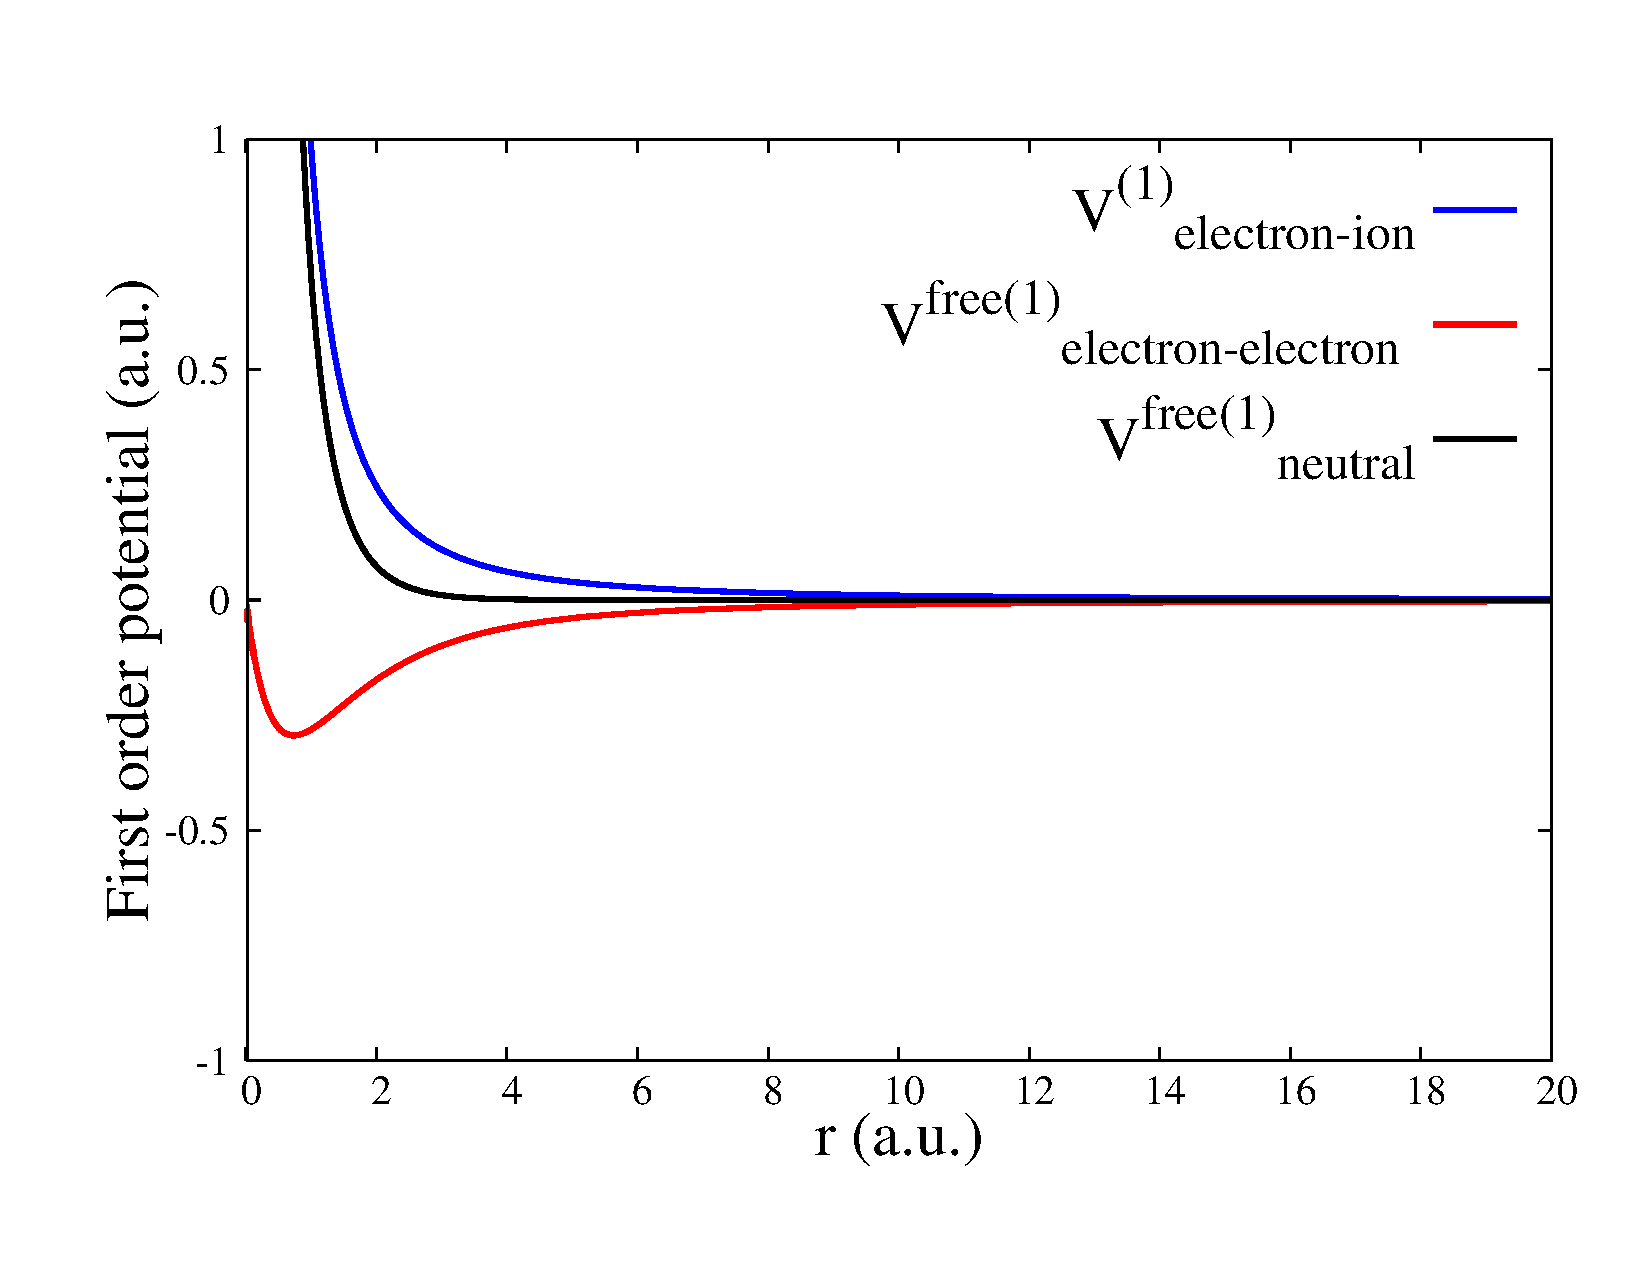
\includegraphics[width=0.7\columnwidth]{why_v_free_1}
 \caption{The screened method for first order potential. Here we use H atom as an example.}
\end{figure}

The general idea of screened scheme is to use free part of electronic Coulomb potential to screening the ion charge Coulomb potential and get short-range neutral potential: 
\begin{align}
V^{free}_{neutral}(|\mathbf{r-R}_I|)= V_{electron-ion} + V^{free}_{electron-electron} \\
=-\dfrac{Z_I}{|\mathbf{r-R}_I|}+\int{\dfrac{n^{free}(\mathbf{r'-R}_I)}{|\mathbf{r-r'}|}d \mathbf{r'}} \nonumber
\end{align}

So the total electrostatic potential can be written as\cite{Blum08}
\begin{align}
V_{es}(\mathbf{r})= -\sum_{Im}\dfrac{Z_{I}}{|\mathbf{r}-\mathbf{R}_{Im}|} +\int{\dfrac{n(\mathbf{r'})}{|\mathbf{r-r'}|}d\mathbf{r'}} \\
=-\sum_{Im}\dfrac{Z_{I}}{|\mathbf{r}-\mathbf{R}_{Im}|} +\int{\dfrac{n^{free}(\mathbf{r'}) + \delta n(\mathbf{r'})    }{|\mathbf{r-r'}|}d\mathbf{r'}} \nonumber \\
= \sum_{I,m}\left[ V^{free}_{neutral}(|\mathbf{r-R}_{I m}|) + \delta V(|\mathbf{r-R}_{I m}|) \right ] 
\end{align}


We follow the line of screened scheme, the first order total electrostatic potential~$V_{es,tot}^{(1)}(\vec{r})$ can be written as
\begin{align}
V_{es,tot}^{(1)}(\mathbf{r}) = -(\sum_{In}\dfrac{Z_{I}}{|\mathbf{r}-\mathbf{R}_{In}|})^{(1)}  +\int{\dfrac{n^{(1)}(\mathbf{r'})}{|\mathbf{r-r'}|}d\mathbf{r'}} \\
=\dfrac{\partial{-(\sum_{I,n}{\dfrac{Z_{I}}{|\mathbf{r}-\mathbf{R}_{In} |} })} }{\partial{\mathbf{R}_{Im}}}   +  \dfrac{\partial{(\int {\dfrac{n^{\text{free}}(\mathbf{r'}) + \delta n(\mathbf{r'})   }{|\mathbf{r}- \mathbf{r'}|}  d\mathbf{r'}})} }{ \partial{\mathbf{R}_{Im}}} \nonumber \\
= \dfrac{\partial V^{\text{free}}(|\mathbf{r-R}_{I m}|)}{\partial{\mathbf{R}_{I m}}}  +\int{\dfrac{\delta n^{(1)}(\mathbf{r'})}{|\mathbf{r-r'}|}d\mathbf{r'}} \nonumber \\
= \dfrac{\partial V^{\text{free}}(|\mathbf{r-R}_{I m}|)}{\partial{\mathbf{R}_{I m}}}  + \dfrac{\partial{ \delta V(\mathbf{r})} }{\partial \mathbf{R}_{Im} } \label{eq:V1_screened} 
\end{align}
In this way, the first order total electrostatic is
divided into two part: free part $\frac{\partial V^{\text{free}}(|\mathbf{r-R}_{I m}|)}{\partial{\mathbf{R}_{I m}}}$ and residual part $\frac{\partial{ \delta V(\mathbf{r})} }{\partial \mathbf{R}_{Im} }$, as shown in Eq. (\ref{eq:V1_screened}).


\subsubsection{Sparse Matrix}
Pleas note that, all matrices in our real-space implementation are in
sparse matrix form. see Fig \ref{fig:PBC_in_FHI-aims}
We choose the matrix elements which is just in touch 
with unit cell basis sets, as labelled by i-place in the middle.

\begin{figure}
\caption{The sparse matrix storage in FHI-aims for overlap matrix, Hamiltonian matrix and density matrix, here is an example for H$_2$-line. In total, there are 13 cells~(i-cell), with cell-index from [-6,0,0] to [6,0,0]. Only centers (i-center) within these cells are considers to build sparse matrix~(i-place), the other original centers are just dropped because of no overlap with unit cell.}
\label{fig:PBC_in_FHI-aims}
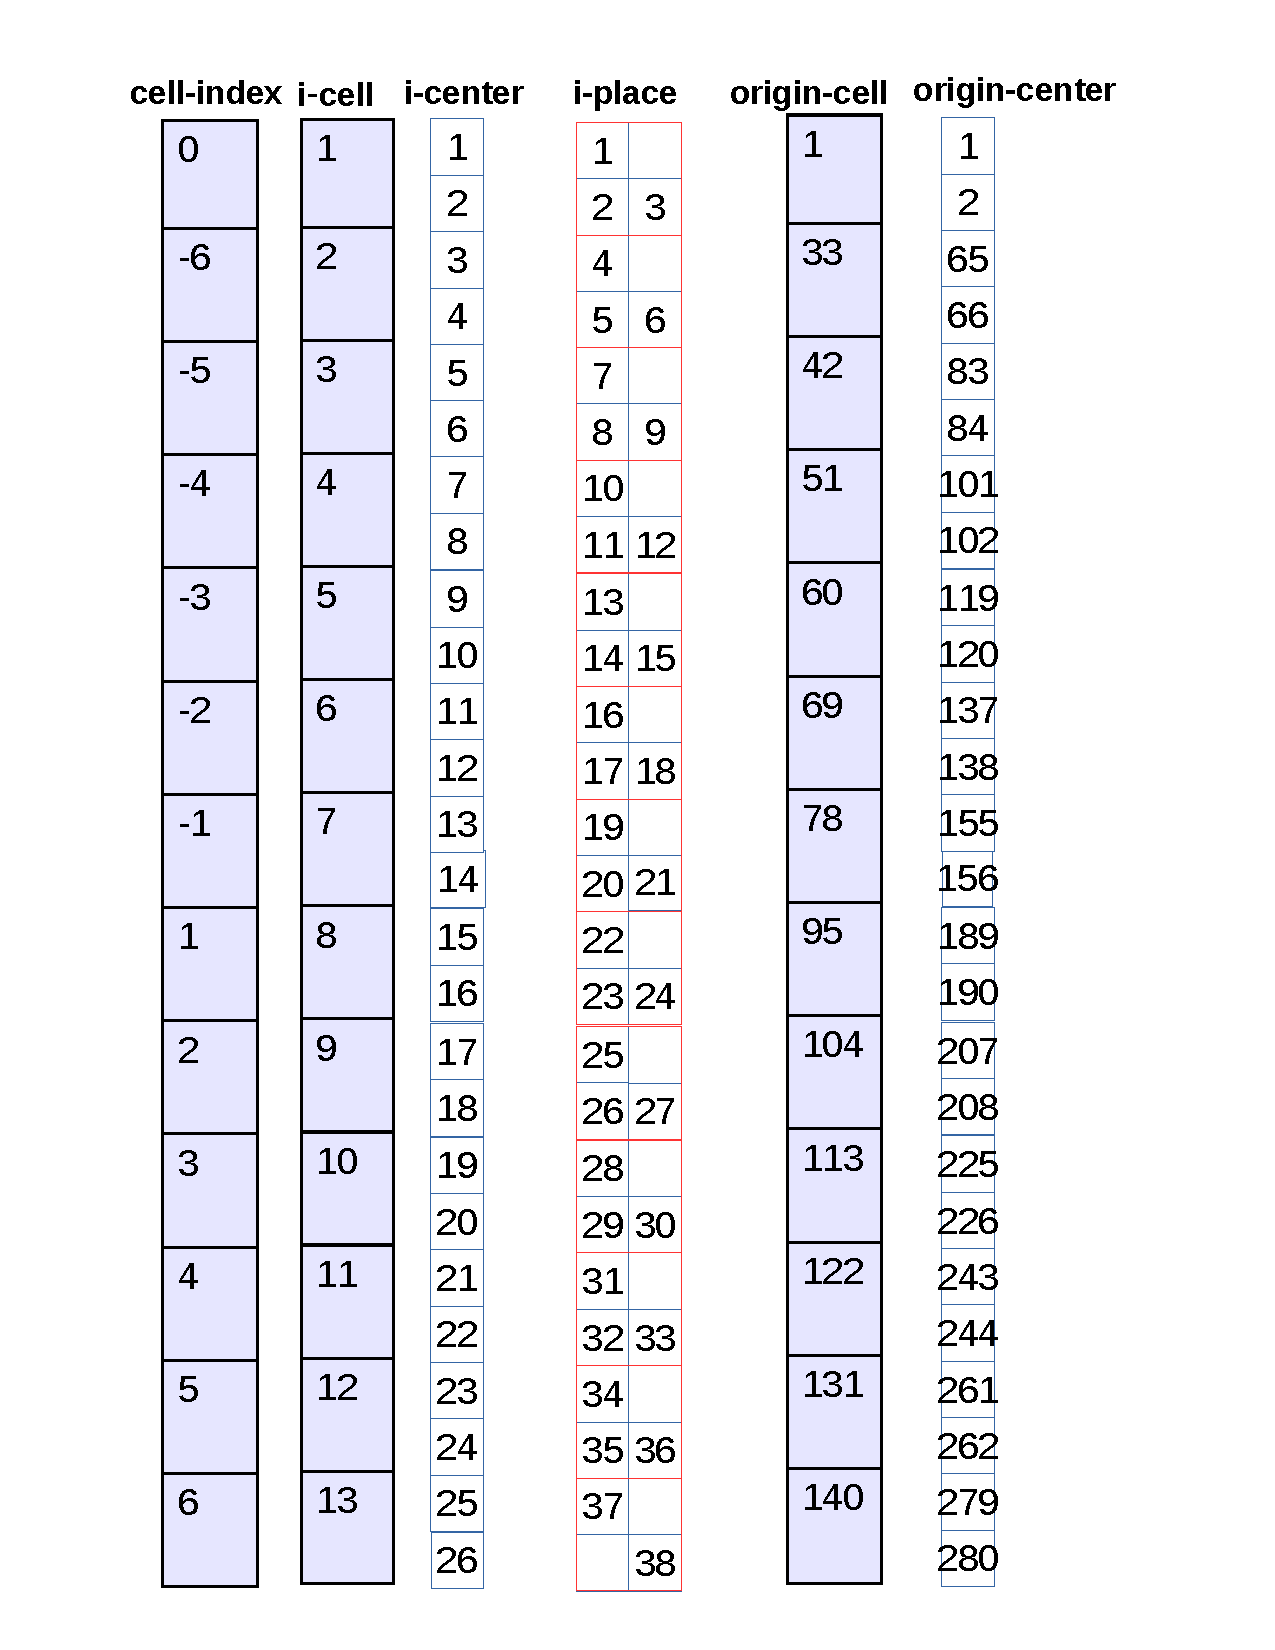
\includegraphics[width=0.7\columnwidth]{PBC_in_FHI-aims.pdf}
\end{figure}

\subsubsection{Using Pulay mixer}
The Pulay mixer is the same as the one used in Magnetic Response. However, in current 
\begin{verbatim} 
DFPT phonon
DFPT phonon_reduce_memory
DFPT polarizability
DFPT dielectric
\end{verbatim}
by default, the Pulay mixer (pulay step 8) is used, and the mixing parameter is set by 
\begin{verbatim}  
   DFPT_mixing   0.2
   DFPT_sc_accuracy_dm   0.001
\end{verbatim}
The Pulay mixer can be changed by writing the number of pulay steps in contron.in. 
\begin{verbatim} 
dfpt_pulay_steps 8
\end{verbatim}

\clearpage

\subsection*{Tags for general section of \texttt{control.in}}
\keydefinition{DFPT vibration}{control.in}
{
Usage: \keyword{DFPT vibration} \option{[subkeywords and their options]}\\[1.0em]
  Purpose:  Allows to calculate vibrations using density-functional perturbation theory, use Acoustic Sum Rule (ASR) to get Hessian matrix, do not use moving-grid-effect.\\


Usage: \keyword{DFPT vibration\_with\_moving\_grid\_effect} \option{[subkeywords and their options]}\\[1.0em]
  Purpose: give the results for vibrations with moving-grid-effect, do not use ASR for Hessian matrix.\\ 

Usage: \keyword{DFPT vibration\_without\_moving\_grid\_effect} \option{[subkeywords and their options]}\\[1.0em]
  Purpose: give the results for vibrations without moving-grid-effect, ONLY served as comparison with vibration\_with\_moving\_grid\_effect.\\ }



\keydefinition{DFPT vibration\_reduce\_memory}{control.in}
{
Usage: \keyword{DFPT vibration\_reduce\_memory} \option{[subkeywords and their options]}\\[1.0em]
  Purpose: Allows to calculate vibrations density-functional perturbation theory by using nearly the same memory as DFT.  At present, functionals LDA, PBE are supported, relativistic is also supported. It should be noted that PBE and PBE+TS is supported only for DFPT cycle (first-order-H), but not for Hessian.  Only linear-mix (no Pulay-mixer) can be used for DFPT vibration\_reduce\_memory at present.\\ }

Here is an example,  the following need to be added to control.in:
\begin{verbatim} 
DFPT vibration_reduce_memory
DFPT_mixing   0.2       #default is 0.2
DFPT_sc_accuracy_dm   1E-6  # default is 1.0d-6
\end{verbatim}  

\keydefinition{DFPT phonon\_gamma}{control.in}
{
Usage: \keyword{DFPT phonon\_gamma} \option{[subkeywords and their options]}\\[1.0em]
  Purpose: Allows to calculate phonon for PBC systems using density-functional perturbation theory. This feather use the dense matrix in FHI-aims, which cost a lot of memory, so this keyword only served as a benchmark for DFPT phonon\_reduce\_memory.  \\ }

\keydefinition{DFPT phonon}{control.in}
{
Usage: \keyword{DFPT phonon} \option{[subkeywords and their options]}\\[1.0em]
  Purpose: Allows to calculate phonon (real space method) for PBC systems using density-functional perturbation theory. This method could get force constants using real space method and give the phonon band structures. At present, only functionals LDA without relativistic is supported.\\ }

Here is an example for using DFPT phonon,  the following need to be added to control.in:
\begin{verbatim} 
DFPT phonon
DFPT_mixing   0.5             #default is 0.2
DFPT_sc_accuracy_dm   1.0d-6  # default is 1.0d-3
dfpt_pulay_steps 6            # default is 8
\end{verbatim}  
  

\keydefinition{DFPT phonon\_reduce\_memory}{control.in}
{
Usage: \keyword{DFPT phonon\_reduce\_memory} \option{[subkeywords and their options]}\\[1.0em]
  Purpose: Allows to calculate phonon (reciprocal space method) at q point for PBC systems using density-functional perturbation theory. At present, this keyword only works to get dynamic matrix at q = 0.  This feature is under developing. At present, functionals LDA, PBE are supported, relativistic is also supported. It should be noted that PBE and PBE+TS is supported only for DFPT cycle (first-order-H), but not for Hessian.\\}

Here is an example for using DFPT phonon\_reduce\_memory,  the following need to be added to control.in:
\begin{verbatim} 
DFPT phonon_reduce_memory
DFPT_mixing   0.5             #default is 0.2
DFPT_sc_accuracy_dm   1.0d-6  # default is 1.0d-3
dfpt_pulay_steps 6            # default is 8
\end{verbatim}  



\keydefinition{DFPT polarizability}{control.in}
{
Usage: \keyword{DFPT polarizability} \option{[subkeywords and their options]}\\[1.0em]
  Purpose: Allows to calculate polarizability for cluster systems using density-functional perturbation theory.\\  For "DFPT polarizability", functionals LDA, PBE, HF(RI-V) are supported, relativistic is also supported.  }
  
Here is an example for using DFPT polarizability,  the following need to be added to control.in:
\begin{verbatim} 
DFPT polarizability
DFPT_mixing   0.5             #default is 0.2
DFPT_sc_accuracy_dm   1.0d-6  # default is 1.0d-3
dfpt_pulay_steps 6            # default is 8
\end{verbatim}  

\keydefinition{DFPT dielectric}{control.in}
{
Usage: \keyword{DFPT dielectric} \option{[subkeywords and their options]}\\[1.0em]
  Purpose: Allows to calculate dielectric constant for extended systems using density-functional perturbation theory. For "DFPT dielectric", functionals LDA, PBE, are supported, relativistic is also supported. }

Here is an example for using DFPT dielectric,  the following need to be added to control.in:
\begin{verbatim} 
DFPT dielectric
DFPT_mixing   0.5             #default is 0.2
DFPT_sc_accuracy_dm   1.0d-6  # default is 1.0d-3
dfpt_pulay_steps 6            # default is 8
\end{verbatim} 


\keydefinition{DFPT\_width}{control.in}
{
Usage: \keyword{DFPT\_width} \option{width}\\[1.0em]
  Purpose: Removes the divergence that can arise in case of small eigenvalue differences and/or fractional occupation numbers.
  This keyword is to employ in combination with a DFPT dielectric calculation. Note that it has not been thoroughly tested, and 
  some small adjustments might be needed.\\[1.0em]
  \option{width} is a real number that corresponds to the width of the smearing function (in eV). A value of 0.01 eV proves reasonable in most cases. \\ [1.0em]
  The usual expressions employed to calculate the 
  first-order quantities fail when tiny eigenvalue differences are present and/or when the system under study has some fractional occupation numbers,
  potentially leading to divergences when calculating the polarizability and dielectric constant.
  In order to circumvent this, we use a similar scheme as the one proposed by de Gironcoli~\cite{Gironcoli95}, which makes use of smearing functions to convolute the density of states.}

